\chapter{GRAMMAIRE GÉNÉRATIVE ET RÉVOLUTION CHOMSKYENNE}
\label{chapter-14}
\markright{Grammaire générative et révolution chomskyenne}
\origpage{425}{411}
\begin{keybox}[Plan du chapitre]
\small\setstretch{1.01}
\setlist{topsep=.12em,itemsep=.12em,parsep=0pt}
\textbf{I.\quad LA LINGUISTIQUE DISTRIBUTIONNALISTE}
\begin{enumerate}[label=\arabic*.]
\item Distributionnalisme et anthropologie\par
\textcircled{\scriptsize 1} Franz Boas : le père de l’anthropologie américaine\par
\textcircled{\scriptsize 2} Léonard Bloomfield : le fondateur du distributionnalisme\par
\textcircled{\scriptsize 3} Edward Sapir : le relativisme linguistique\par
\textcircled{\scriptsize 4} Zellig Harris\par\hspace*{1em}1. Les prémices de l’analyse transformationnelle\par\hspace*{1em}2. Professeur et mentor de Chomsky
\item Distributionnalisme et béhaviorisme\par
\textcircled{\scriptsize 1} John Broadus Watson : le fondateur\par\hspace*{1em}1. Le rejet du « mentalisme »\par\hspace*{1em}2. L’expérience du petit Albert\par
\textcircled{\scriptsize 2} Burrhus Skinner : le comportement verbal\par\hspace*{1em}1. La boîte de Skinner\par\hspace*{2em}1) La notion de conditionnement opérant\par\hspace*{2em}2) Les notions de renforcement et de punition\par\hspace*{2em}3) Les quatre types de comportements opérants\par\hspace*{1em}2. \textit{Verbal behaviour} (1957)\par\hspace*{2em}1) Les postulats de base\par\hspace*{2em}2) Les opérants verbaux\par\hspace*{2em}3) Comportement verbal et traitement de l’autisme\par\hspace*{1em}3. La critique de Chomsky
\item L’analyse distributionnaliste\par
\textcircled{\scriptsize 1} Les postulats de base\par\hspace*{1em}1. Une théorie mécaniste\par\hspace*{1em}2. Une théorie asémantique\par
\textcircled{\scriptsize 2} L’analyse en constituants immédiats\par\hspace*{1em}1. La segmentation\par\hspace*{1em}2. La commutation\par\hspace*{1em}3. La notion de syntagme\par\hspace*{1em}4. Hiérarchie des constituants immédiats
\end{enumerate}
\origpage{426}{412}
\textcircled{\scriptsize 3} Les représentations graphiques\par\hspace*{1em}1. Les arborescences\par\hspace*{1em}2. Les boîtes de Hockett\par\hspace*{1em}3. Le parenthésage étiqueté\par
\textcircled{\scriptsize 4} Les limites du modèle

\textbf{II.\quad LA GRAMMAIRE GÉNÉRATIVE TRANSFORMATIONNELLE}
\begin{enumerate}[label=\arabic*.]
\item La critique et dépassement du modèle distributionnaliste\par
\textcircled{\scriptsize 1} Un triple rejet\par\textcircled{\scriptsize 2} Première critique\par\textcircled{\scriptsize 3} Deuxième critique\par\textcircled{\scriptsize 4} Troisième critique
\item La Théorie Standard\par
\textcircled{\scriptsize 1} Une approche modulaire\par\textcircled{\scriptsize 2} Structure profonde et structure de surface\par\textcircled{\scriptsize 3} Compétence et performance\par\textcircled{\scriptsize 4} Les règles de réécriture (rewriting rules)\par\textcircled{\scriptsize 5} Les règles transformationnelles\par\hspace*{1em}1. La notion de transformations syntaxiques\par\hspace*{1em}2. Les différents types de transformations\par\hspace*{2em}1) Transformation interrogative\par\hspace*{2em}2) Transformation passive\par\hspace*{2em}3) Transformation négative\par\hspace*{1em}3. Les procédés morphosyntaxiques de transformation
\item La Théorie Standard Étendue\par
\textcircled{\scriptsize 1} La Théorie des X-barres\par\textcircled{\scriptsize 2} \textit{Conditions on Transformations}
\item Les Principes et Paramètres (P\&P)\par
\textcircled{\scriptsize 1} \textit{Lectures on Government and Binding}\par\hspace*{1em}1. Liage et catégorie gouvernante\par\hspace*{1em}2. Les trois principes du liage\par\hspace*{2em}1) Le principe A : l’anaphore\par\hspace*{2em}2) Le principe B : le pronom\par\hspace*{2em}3) Le principe C : l’expression référentielle\par
\textcircled{\scriptsize 2} La Théorie des Barrières (subjacency theory)\par\hspace*{1em}1. Le mouvement Qu (WH-movement)\par\hspace*{1em}2. Sous-jacence et îlots syntaxiques (Wh islands)\par
\textcircled{\scriptsize 3} P-structure et S-structure\par\textcircled{\scriptsize 4} Modules intentionnel-conceptuel et sensori-moteur
\origpage{427}{413}
\item Le programme minimaliste (Minimalist Program)\par
\textcircled{\scriptsize 1} La numération\par\textcircled{\scriptsize 2} La fusion (merge)\par\textcircled{\scriptsize 3} Le déplacement (move) et la vérification (feature-checking)\par\textcircled{\scriptsize 4} L’épellation (spell-out)
\end{enumerate}
\textbf{Exercices}\par\textbf{Pour aller plus loin}\par\textbf{Glossaire}
\end{keybox}

\origpage{428}{414}
\begin{keybox}[Introduction]
Au début des années 50, la linguistique américaine est en plein essor. En 1955, le linguiste \textbf{Henry Allan Gleason} parle des « résultats définitifs obtenus par la linguistique structurale, qui, par sa méthode, peut se comparer à la physique, à la mécanique quantique, aux mathématiques ». Si cette période constitue un certain âge d’or dans la linguistique américaine, on peut distinguer deux orientations principales :

\begin{itemize}[leftmargin=1.5em]
\item Un courant d’inspiration structuraliste, préoccupé d’ethnolinguistique, s’est développé à partir des travaux de Leonard Bloomfield et a dominé la linguistique américaine jusqu’au à début des années 1950.\ednote{Le groupe « jusqu’au à début » cumule deux constructions. La forme attendue est « jusqu’au début ». Le texte de base est conservé.} Ce structuralisme américain d’inspiration bloomfieldienne s’est concentré sur les phénomènes de distribution à l’intérieur de la chaîne parlée (d’où son nom de distributionnalisme) et a donné la priorité à l’étude de la structure syntagmatique du langage.
\item Dès la fin des années 1950, on a assisté à l’émergence d’une linguistique générative en réaction contre ces approches structuralistes et dont l’initiateur principal est Noam Chomsky. Sa \textit{generative grammar} est une grammaire formelle destinée à rendre compte du savoir linguistique des locuteurs (\textit{competence}) par sa capacité à énumérer l’ensemble infini des phrases grammaticales d’une langue au moyen d’un ensemble fini de règles (\textit{rewriting rules}). \textit{Aspects of the Theory of Syntax} (1965), Chomsky la définit ainsi :\ednote{Après le titre d’ouvrage, la phrase appelle une préposition : « Dans \textit{Aspects of the Theory of Syntax} (1965), Chomsky la définit ainsi ».}
\end{itemize}
\begin{lecture}{Aspects of the Theory of Syntax (1965)}
A grammar of a language purports to be a description of the ideal speaker-hearer’s intrinsic competence. If the grammar is, furthermore, perfectly explicit—in other words, if it does not rely on the intelligence of the understanding reader but rather provides an explicit analysis of his contribution—we may (somewhat redundantly) call it a generative grammar.
\end{lecture}
La linguistique américaine possède aussi ses caractères spécifiques par rapport à la linguistique européenne : grand souci de description effective, attention portée aux langues parlées sans tradition écrite, méfiance à l’égard de la sémantique « mentaliste », recours à des techniques mathématiques de segmentation, de distribution, de fréquence.
\end{keybox}

\section{LA LINGUISTIQUE DISTRIBUTIONNALISTE}
Une des caractéristiques de la linguistique américaine est son côté pratique. Au moment où est né le distributionnalisme, c’est-à-dire dans les années 1920, linguistes et anthropologues américains commençaient à s’intéresser aux langues amérindiennes. Or, ces dernières, en plus de ne pas posséder de langage écrit, sont génétiquement très éloignées des langues indo-européennes comme le latin, le grec ou l’anglais. Les outils et méthodes de la linguistique européenne étant inutilisables, il a donc fallu mettre au point une nouvelle méthode et de nouvelles procédures pour analyser et comprendre la structure de ces langues indigènes. Cette méthode, que l’on verra un peu plus tard, est appelée « analyse en constituants immédiats ». En quelques

\origpage{429}{415}

mots, elle consiste à partir d’un énoncé, de le segmenter de façon à obtenir, par segmentation successives, ses éléments constitutifs minimaux, qui ne sont rien d’autre que des morphèmes : cela devrait vous rappeler le fonctionnalisme. Prenons une image : si l’énoncé est une maison, alors il s’agit de la déconstruire pour obtenir des briques, puis d’étudier leur distribution, c’est-à dire la façon dont on peut les combiner. La distribution est une notion de statistique : il faut la comprendre ici comme l’environnement d’un morphème, à savoir sa place dans l’énoncé, relativement aux autres morphèmes qui précèdent ou le suivent.\par

\subsection{Distributionnalisme et anthropologie}
Une des conséquences directes du contexte d’apparition de la linguistique distributionnaliste est qu’elle est fortement imprégnée d’ethnologie. Les linguistes structuralistes étaient tous anthropologues de formation.\par

\minititle{\textcircled{\scriptsize 1} Franz Boas : le père de l’anthropologie américaine}

Franz Boas (1858-1942), anthropologue américain d’origine allemande, est considéré comme le fondateur de l’anthropologie américaine. Opposé à l’évolutionnisme, dissociant l’étude des races de celle des cultures, Boas est considéré comme le père du relativisme culturel : pour lui, aucune culture n’est plus développée qu’une autre. Spécialiste des cultures amérindiennes mais aussi esquimaux, il publié en 1911 un Dictionnaire des langues amérindiennes. Son travail d’ethnologue a eu un retentissement considérable en linguistique, et deux de ses étudiants, Leonard Bloomfield et Edward Sapir, comptent parmi les plus grandes figures de la linguistique américaine.\par

\minititle{\textcircled{\scriptsize 2} Léonard Bloomfield : le fondateur du distributionnalisme}
Linguiste et anthropologue américain, Léonard Bloomfield (1887-1949) a grandement contribué au développement de la linguistique structurale aux États-Unis dans le courant des années 1930 et 1940. Dans le chapitre 9, on a déjà vu ses conceptions sur la notion de connotation, mais c’est en tant que père fondateur du distributionnalisme qu’il est entré dans l’histoire de la linguistique.\par

En 1914, Bloomfield a publié un ouvrage qui fera date : An Introduction to the Study of Language, qui sera réédité en 1933 sous le titre de Language. En 1917, il publie des recherches sur le tagalog, cette langue des Philippines que nous avons rencontrée dans le chapitre 9 (Morphologie). Au début des années vingt, il a commencé à s’intéresser aux langues amérindiennes, en particulier à celles du groupe algonquin\origfoot{1}{En particulier le fox, le cree, le menominee, et l’ojibwa.}. Ses talents de descripteur et sa formation de comparatiste lui ont permis de produire une œuvre qui, avec les travaux de ses grands contemporains Boas et Sapir, sont de nos jours des classiques de ce domaine : il s’agit des Menomini Texts (1928), des Plains Cree Texts (1934), et de son célèbre ouvrage Linguistic Structures of Native America (1946). En 1940, il a succédé à Edward Sapir à la chaire de linguistique de l’université Yale, où il a enseigné jusqu’à sa mort.\par

Cofondateur en 1924 de la Linguistic Society of America puis de la revue Language (1925), Bloomfield est parfois appelé le « Saussure américain ». Ceci est à relativiser : si en effet les\par

\origpage{430}{416}

théories distributionnalistes, nous allons le voir plus bas, ont beaucoup de points communs avec le structuralisme, elles sont cependant apparues aux États-Unis alors que les thèses de Ferdinand de Saussure commençaient à peine à être connues en Europe et étaient inconnues aux États-Unis : le distributionnalisme doit être considéré comme une théorie originale et indépendante par rapport à la pensée de Saussure.\par

Bloomfield est l’auteur de la théorie distributionnaliste des « constituants immédiats » qui reste la base de presque tous les travaux américains contemporains dans le domaine de la syntaxe. Si ses travaux ont conduit à un essor de la linguistique américaine, l’influence de la linguistique structurale bloomfieldienne a progressivement décliné dans les années 1950 et 1960, tandis que la théorie de la grammaire générative développée par Noam Chomsky prenait son essor.\par

\minititle{\textcircled{\scriptsize 3} Edward Sapir : le relativisme linguistique}

Linguiste et anthropologue américain, Edward Sapir (1884-1939) est la figure incontournable de la linguistique structurale américaine. À l’Université de Columbia, Sapir a d’abord fait des études d’allemand, d’anthropologie et de linguistique avant de se spécialiser dans les langues amérindiennes. Il a également beaucoup travaillé sur le problème de la typologie des langues. Refusant le classement génétique proposé par le linguiste français Antoine Meillet dans Les Langues du monde (1924), il a tenté d’élaborer des principes typologiques qui prennent en compte le plus grand nombre possible de données (morphologie, composition, dérivation, organisation sémantique, etc.). Cette nouvelle typologie, inaugurée par Sapir, a beaucoup influencé les travaux de Joseph Greenberg sur les langues africaines. En 1931, il a rencontré Benjamin Lee Whorf à Yale. Ils y ont travaillé ensemble sur la théorie de la relativité linguistique : c’est la célèbre hypothèse de Sapir-Whorf.\par

Aujourd’hui, Sapir est surtout très connu pour cette hypothèse. Pour lui, chaque langue constitue une certaine vision du monde, et le monde réel n’existe qu’à travers ce que notre langue nous en fournit comme vision. Autrement dit, la langue que l’on parle structure la façon dont on voit le monde.\par

L'hypothèse de Sapir-Whorf, nous l’avons vue dans le chapitre 5, avait déjà été formulée au 18° siècle par le linguiste allemand Wilhelm von Humboldt, et avant lui par Johann Gottfried von Herder (1744-1803). Après la mort de Sapir, son étudiant Benjamin Lee Whorf (1897-1941) a étendu et radicalisé cette thèse. Se fondant sur ses recherches et ses observations de terrain sur les langues amérindiennes\origfoot{2}{En particulier les langues hopi, maya et inuit.}, il a suggéré en se basant sur le fait qu’il n’existe aucune notion temporelle dans la langue Hopi, et que la conception du temps et de la ponctualité dans un peuple peut être influencée par les types de temps verbaux que présente sa langue. Whorf en a conclu que la formulation des idées est influencée par la grammaire propre et diffère donc d’une langue à l’autre.\par

\origpage{431}{417}

\minititle{Henri Allan Gleason : la perception des couleurs}

Le langage opère donc un véritable découpage du monde en installant des limites entre les objets. Dans son Introduction à la linguistique (1969), Henry Allan Gleason, linguiste et professeur à l’Université de Toronto a pris un exemple désormais célèbre pour illustrer le relativisme linguistique : les couleurs de l’arc-en-ciel. En voici un extrait :\par

\lecturetitle{Introduction à la linguistique, Henri Allan Gleason}

Considérons un arc-en-ciel ou le spectre d’un prisme. Sur la bande colorée, le passage d’une couleur à l’autre est progressif, c’est-à-dire qu’en chaque point il n’y a qu’une toute petite différence de couleur avec les points immédiatement voisins. Et cependant un Français qui décrit l’arc-en-ciel parle de teintes telles que le rouge, l’orange, le jaune, le vert, le bleu, l’indigo la langue découpe la gradation continue de couleur en une série de catégories discrètes. C’est un exemple de structuration du contenu. Rien dans le spectre ou dans la perception qu’en à l’homme n’oblige à le diviser ainsi. Cette méthode spécifique de division fait partie de la structure du français. Les sujets qui parlent d’autres langues classent les couleurs de bien d’autres manières. Le diagramme suivant donne une idée de la façon dont ceux qui parlent le français, le shona (langue de la Zambie), le bassa (langue du Libéria), divisent le spectre :\par

\begin{center}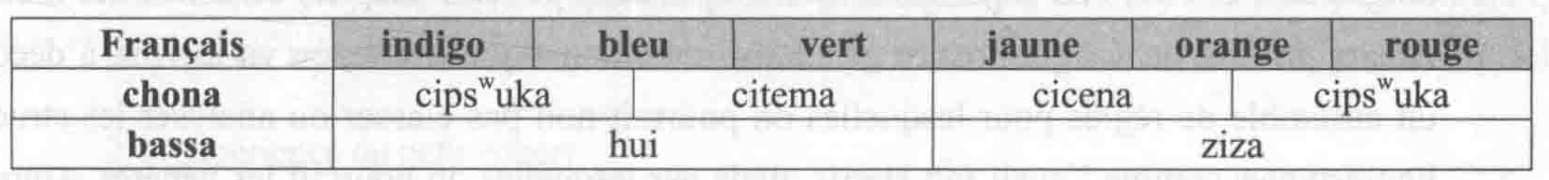
\includegraphics[width=.84\textwidth,height=.29\textheight,keepaspectratio]{assets/v17_colors.png}\end{center}

Le sujet qui parle le chona divise le spectre en trois grandes catégories : si le terme cipswuka revient deux fois, c’est seulement parce que les extrémités rouge et indigo sont rangées dans la même catégorie, même si elles sont distinctes sur le diagramme. Le sujet qui parle le bassa divise quant à lui le spectre de façon radicalement différente en deux catégories seulement. Si dans ces deux langues, il y a beaucoup de mots pour désigner les couleurs spécifiques (comme en français on a écarlate, vermillon, pourpre, qui sont des variétés de rouge) mais il n’existe que trois termes en chona et deux termes en bassa pour les classes générales de couleurs.\par

Pour Gleason, la convention qui consiste à diviser le spectre en deux ou trois parties au lieu de six pour un français ne provient pas d’une différence dans la perception visuelle des couleurs, mais représente seulement une différence dans la manière dont la langue classe ou structure les couleurs.\par

\minititle{\textcircled{\scriptsize 4} Zellig Harris : un pont entre Bloomfield et Chomsky}
Disciple de Léonard Bloomfield, Zellig Harris (1909-1992) est un linguiste américain d’origine ukrainienne connu pour ses travaux sur la linguistique structuraliste et l’analyse du discours. En 1946, c’est également lui qui a fondé le premier département de linguistique dans une université américaine. Refusant toute utilisation du sens comme critère de définition formelle des phonèmes et des morphèmes, Harris l’a remplacé par un critère formel : celui de « distribution », c’est-à-dire\par



\origpage{432}{418}

la somme totale des environnements d’un élément abstrait. Dans son oeuvre majeure, Methods in Structural Linguistics (1951), Harris a appliqué cette méthode distributionnelle à l’analyse phonologique et syntaxique de la phrase. Nous reviendrons longuement sur cet asémantisme, caractéristique essentielle du distributionnalisme.\par

\minititle{1. Les prémices de l’analyse transformationnelle}

Par la suite, dépassant le cadre de la phrase isolée, Harris s’est intéressé à l’analyse du discours dans Discourse Analysis Reprints (1963). Son essai postule qu’on ne peut mener à bien l’analyse du discours sans examiner les rapports entre les phrases qui le constituent. Or, puisqu’il existe en général plusieurs façons de dire la même chose, c’est-à-dire plusieurs paraphrases possibles d’une seule phrase, il n’est pas possible d’analyser systématiquement un discours sans avoir préalablement mis en relation les paraphrases des divers schémas de phrases. C’est l’étude de ces paraphrases, et en particulier le passage d’une paraphrase à une autre que Harris nomme analyse transformationnelle. Harris a exposé sa théorie dans deux articles publiés dans la revue Language : Discourse Analysis (1952), et Co-occurrence and Transformation in Linguistic Structure (1957).\par

\minititle{2. Professeur et mentor de Chomsky}

C’est Zellig Harris qui a initié Chomsky, un de ses étudiants à l’Université de Pennsylvanie, à la linguistique structurale. Il l’a autorisé à lire les épreuves de son livre Methods in Structural Linguistics, et c’est cela a permis à Chomsky d’adopter (et d’adapter) certaines des méthodes de son professeur. La grammaire générative de Chomsky cherche, on va le voir, à découvrir un ensemble de règles pour lesquelles on pourrait non pas classer ou analyser les structures linguistiques comme l’avait fait Harris, mais par lesquelles on pourrait les générer. Autrement dit, pour reprendre notre image, partir des constituants minimaux (les briques) pour construire un énoncé (une maison). Notez aussi, pour rendre à César ce qui est à César, que c’est dans un manuscrit de Harris daté de Janvier 1946 qu’apparaît pour la première fois la notion de\par

« generative grammar ».\par

En 1955, Chomsky a rédigé terminé un manuscrit\ednote{La suite « a rédigé terminé » superpose deux verbes. On attend soit « a rédigé un manuscrit », soit « a terminé un manuscrit ». Le texte de base est maintenu.} de mille pages, The logical structure of linguistic theory dont le neuvième chapitre, Transformational analysis lui a servi d’abord de thèse de doctorat avant de devenir un élément central de son modèle génératif. Nous y reviendrons en temps voulu, mais revenons dans l’immédiat au distributionnalisme qui entretient des liens très proches avec l’ethnologie mais aussi avec la psychologie comportementaliste appelée béhaviorisme.\par

\subsection{Distributionnalisme et béhaviorisme}

Le béhaviorisme est une théorie psychologique basée sur l’étude du comportement observable et qui s’appuie sur l’expérimentation et les mesures scientifiques. Le distributionnalisme, né de ce mariage entre linguistique et béhaviorisme, considère les faits de langue du point de vue du comportemental : dans cette optique, le langage est un comportement humain mécanique et explicable.\par

\origpage{433}{419}

\minititle{\textcircled{\scriptsize 1} John Broadus Watson : le fondateur}
L’acte de naissance du béhaviorisme est un article du psychologue américain John Broadus Watson (1878-1958), publié en 1913 dans la Psychological Review, revue dirigée par lui-même, et intitulé « Psychology as the Behaviorist Views it ». Il a ensuite développé ses idées dans divers articles et ouvrages, dont le principal est Behaviorism (1925).\par

\minititle{1. Le rejet du « mentalisme »}

Voulant faire de la psychologie « une science de la nature » aussi objective que la médecine, la chimie ou la physique, Watson défend l’idée que celle-ci doit se cantonner à l’étude rigoureuse des comportements (behavior, en anglais) observables, tels qu’ils se produisent en réponse à un stimulus. Dans Le Behaviorisme, il écrit :\par

Pourquoi ne pas faire de ce que nous pouvons observer le champ réel de la psychologie ? Limitons-nous aux choses qui peuvent être observées et formulons des lois concernant uniquement ces choses. Cette limitation a fondé effectivement la psychologie scientifique qui rejette toute référence non seulement à des entités métaphysiques telles que l’âme ou l’esprit, ou à la conscience mais refuse aussi de considérer les états mentaux comme des objets d’observation. En ce qui nous concerne, c’est-à-dire du point de vue linguistique, le prolongement de cette prise de position est que le langage est lui-même considéré comme un comportement et qu’il doit être analysé comme tel.\par

\minititle{2. L'expérience du petit Albert}

Dans le droit fil des travaux d’Ivan Pavlov, lauréat du prix Nobel de physiologie ou médecine de 1904 et célèbre pour ses travaux sur les réflexes conditionnés, Watson accorde une place centrale aux phénomènes de conditionnement, de stimulus et de réponse. Son expérience la plus célèbre, dite « expérience du petit Albert » avait pour but de conditionner un bébé de sorte qu’il ait peur d’un rat blanc, qu’il ne craignait pas du tout au préalable. Pour ce faire, Watson a repris la théorie du conditionnement simple animaux d’Ivan Pavlov. Watson présentait le rat au petit Albert, et a chaque fois qu’il le touchait, on produisait un son violent en frappant une barre métallique avec un marteau pour effrayer le bébé. Au bout de quelques répétitions, le petit Albert a fini par avoir peur du rat, rien qu’en le voyant, de la même façon que chien de Pavlov salivait en entendant la cloche de son maître. Watson a ainsi pu prouver que le conditionnement simple, qui n’avait été observé que chez les animaux, pouvait également s’appliquer aux humains.\par

\minititle{\textcircled{\scriptsize 2} Burrhus Skinner : le comportement verbal}
Fondateur du béhaviorisme radical, Burrhus Skinner (1904-1990) est fortement influencé par les travaux de Pavlov et de Watson. En 1990, l’ Association Américaine de Psychologie lui a décerné le titre de « psychologue le plus important du siècle ». Son nom reste associé de nos jours a son expérience de la « boîte de Skinner » et à son ouvrage majeur, Verbal behaviour.\par

\origpage{434}{420}

\minititle{1. La boîte de Skinner}

La boîte de Skinner est une cage conçue par Skinner au début des années 1930 pour étudier le conditionnement opérant des animaux.\par

\minititle{1) La notion de conditionnement opérant}

Si, depuis Pavlov, nous connaissons la notion de conditionnement, le conditionnement « opérant » de Skinner désigne la façon dont un comportement opère sur son environnement. Pour l’étudier, Skinner a inventé un dispositif pour tester et observer les capacités de rats ou de pigeons à subir un conditionnement opérant (appelé aussi apprentissage skinnerien). Faisant intervenir le comportement de l’animal et le renforcement de comportement par des stimuli renforçateurs, la boîte de Skinner comporte donc un dispositif de présentation de stimulus (visuel, auditif ou électrique), un dispositif de réponse de l’animal à ces stimulus (un levier), et distributeur de nourriture.\par

\minititle{2) Les notions de renforcement et de punition}

L'apprentissage skinnerien repose sur le renforcement (procédé qui augmente la probabilité de répétition d’un comportement) et la punition (procédé qui rend moins probable répétition d’un comportement). Le renforcement et la punition peuvent être positif (ajout d’un stimulus) ou négatif (retrait d’un stimulus). Le renforcement positif consiste, par exemple, à soumettre l’animal à un stimulus agréable qui augmentera la fréquence d’apparition d’un comportement. À l'inverse, le renforcement négatif consiste à supprimer un stimulus.\par

\minititle{3) Les quatre types de comportements opérants}

Les expériences de Skinner sur les rats ont mis en évidence quatre types de conditionnements opérants, décrits ci-dessous :\par

Le renforcement positif :\par

Stimulus : Le rat est dans la cage.\par

Réponse : Le rat appuie sur le levier. (comportement)\par

Renforcement positif : Il obtient de la nourriture. (ajout d’un stimulus)\par

— Augmentation de la probabilité d’apparition du comportement\par

Le renforcement négatif :\par

Stimulus : Le rat dans la cage reçoit des chocs électriques.\par

Réponse : Le rat appuie sur le levier. (comportement)\par

Renforcement négatif : Les chocs électriques s’arrêtent. (retrait d’un stimulus)\par

— Augmentation de la probabilité d’apparition du comportement\par

\origpage{435}{421}

La punition positive :\par

Stimulus : Le rat est dans la cage.\par

Réponse : Le rat appuie sur le levier. (comportement)\par

Punition positive : Il reçoit une décharge électrique. (ajout d’un stimulus) — Diminution de la probabilité d’apparition du comportement\par

La punition négative :\par

Stimulus : Le rat dans la cage a de la nourriture.\par

Réponse : Le rat appuie sur le levier. (comportement)\par

Punition négative : La nourriture disparaît. (retrait d’un stimulus)\par

— Diminution de la probabilité d’apparition du comportement\par

\minititle{2. Verbal behaviour (1957)}

Les béhavioristes préfèrent parler de « comportements verbaux » plutôt que de langage, et Skinner a développé sa vision comportementale des comportements verbaux dans livre important, Verbal\par

Behavior (1957), qui est une analyse théorique du comportement linguistique du point de vue scientifique.\par

\minititle{1) Les postulats de base}

Pour Skinner, le comportement verbal obéit aux mêmes règles que les autres comportements, avec une différence toutefois : il n’est pas directement renforcé par l’environnement physique, mais de façon indirecte, par le comportement des autres personnes :\par

\begin{lecture}{Extrait}
Un comportement verbal est un comportement renforcé par la médiation d’autres personnes.
\end{lecture}

Skinner distingue également les comportements qui « modifient l’environnement d’une façon mécanique » et les comportements verbaux qui n’agissent pas directement sur l’environnement, mais sur une autre personne :\par

\begin{lecture}{Extrait}
Le comportement verbal est mis en forme et conservé par un environnement verbal par des personnes qui répondent au comportement de certaines manières en raison des pratiques du groupe dont ils font partie. Ces pratiques et l'interaction qui en résulte, entre celui qui parle et celui qui écoute, génèrent les phénomènes qui sont considérés ici sous la rubrique du comportement verbal.
\end{lecture}

\minititle{2) Les opérants verbaux}

L'approche de Skinner a la particularité d’être fonctionnelle : différents comportements\par

\origpage{436}{422}

verbaux peuvent être définis en fonction des stimuli qui contrôlent leur apparition et du type de conséquences qu’ils engendrent. Le même mot pouvant avoir plusieurs fonctions suivant le contexte dans lequel on l’utilise, Skinner distingue six verbal operants (« opérants verbaux ») pour l’utilisation d’un mot, en prenant compte leur fonction sur l’environnement, autrement dit le type de renforcement obtenu. Je présente ci-dessous les trois les plus importants :\par

Le mand (aphérèse de l’anglais command, demand), lorsqu’un mot est utilisé pour demander. C’est le premier comportement verbal acquis chez l’enfant. Skinner note qu’il existe souvent un lien entre le mand et l’état de l’organisme : déprivation, satiété, faim, soif, etc. Par exemple, un enfant qui veut un pain au chocolat demandera : « un pain au chocolat ! »\par

Le Tact est l’aphérèse de contact dans « the behavior makes contact with the physical world », c’est-à-dire « le comportement crée un contact avec le monde physique ». Un enfant passant devant une boulangerie et voyant un pain au chocolat s’écrira : « un pain au chocolat ! »\par

L’Intraverbal fait référence à l’utilisation d’un mot dans une conversation. « Que voulez- vous manger après avoir fini la lecture de ce chapitre ? » Réponse : « Un pain au chocolat ! »\par

Pour Skinner, les intraverbaux sont, avec les mands et les tacts, les opérants verbaux les plus importants : le fait qu’ils soient bien développés chez une personne permet une amélioration des compétences sociales et conversationnelles. 3) Comportement verbal et traitement de l’autisme\par

Parce qu’elle est liée aux compétences sociales et conversationnelles, la théorie des opérants verbaux de Skinner est utilisée de nos jours pour traiter les troubles comportementaux chez l’enfant, en particulier dans les cas d’autisme.\par

C’est par les demandes qu’un enfant entre dans la communication. C’est pour cette raison que la thérapie commence toujours par l’enseignement des mand.\par

Dès qu’un enfant a acquis un bon répertoire de mand, le thérapeute aborde le travail du tact. En nommant, un enfant réagit 4 son environnement, qu’il soit visuel, sonore ou physique. Par exemple : « Voiture ! », « Le chat ! », « C’est chaud ! ». Ce travail sur le tact se fait en posant à l’enfant la question « Qu’est-ce-que c’est ? » et en lui montrant un objet ou une image. L’enfant réagit en nommant l’objet par une parole ou par un signe.\par

Dès que l’enfant a un répertoire de 300 mots sous forme de demandes ou de tact, il devient possible de l’entraîner à la conversion, domaine de l’intraverbal.\par

Des renforçateurs sont également utilisés pour fournir à l’enfant une conséquence agréable lorsqu’il adopte un comportement que l’on souhaite développer chez lui. Il s’agit des renforçateurs sociaux (félicitations, encouragements, calins, etc.), sensoriels (jouets ou objets stimulant les sens de l’enfant), et alimentaires (bonbons, etc.).\par

\origpage{437}{423}

\minititle{3. La critique de Chomsky}

Skinner, qui a beaucoup publié, considérait son Verbal behaviour comme son ouvrage le plus important. Or, dès sa parution, il a fait l’objet de nombreuses critiques de linguistes mais aussi de comportementalistes reprochant à son ouvrage de ne se baser que sur l’interprétation de comportements observés, et donc de ne pas avoir de bases scientifiques. La critique la plus virulente est venue de Noam Chomsky. Dans un article intitulé A review of B. F Skinners Verbal Behavior publié en 1957 dans la revue Language\ednote{La recension de Chomsky, « A Review of B. F. Skinner’s Verbal Behavior », a paru dans \textit{Language}, vol. 35, no 1, en 1959, et non en 1957. 1957 est l’année de publication du livre de Skinner.}, le jeune Chomsky reprend cette critique, dont quelques extraits ci-dessous de la version française publiée en 1969 dans la revue Langages :\par

\begin{lecture}{A review of B. F. Skinner’s Verbal Behavior (extraits)}
« Quand on ne dispose pas de données neurophysiologiques indépendantes, il est évident que les conclusions concernant la structure de l’organisme sont fondées sur l’observation du comportement et des événements extérieurs. [...] Ceci crée l’illusion d’une théorie scientifique rigoureuse de portée très générale, bien qu’en fait la description du comportement de tous les jours et celui du laboratoire puissent être de simples homonymes. [...] »
\end{lecture}

Chomsky souligne que découvertes de Skinner reposent sur des hypothèses discutables, et que ses résultats ne sont pas transposables au comportement humain :\par

\begin{lecture}{Suite}
« L’étude minutieuse de ce livre (et de la recherche qui le sous-tend) révèle que ces hypothèses surprenantes sont loin d’être justifiées. Elle montre de plus que les découvertes brillantes que ce théoricien du renforcement a faites dans ses laboratoires, bien qu’authentiques, ne s’appliquent au comportement humain complexe que de manière très grossière et très superficielle. »
\end{lecture}

Une autre critique est d’ordre conceptuel et concerne les notions de stimulus, de réponse, et renforcement, qui sont au cœur de la théorie de Skinner :\par

\begin{lecture}{Suite}
« Avant de pouvoir les étendre au comportement de la vie réelle, il faut résoudre un certain nombre de problèmes. »
\end{lecture}

La conclusion de ce très long article, dont on n’a lu que quelques courts extraits, est sans appel :\par

\begin{lecture}{Suite}
« Tout chercheur qui aborde sérieusement l’étude du comportement linguistique, qu’il soit linguiste, psychologue ou philosophe, s’aperçoit rapidement de la difficulté considérable qu’il y a à définir un problème qui constitue le domaine de ses recherches et tel qu’il ne soit ni trop banal ni hors d’atteinte dans l’état actuel de la connaissance et de la technique. En choisissant pour problème l’analyse fonctionnelle, Skinner s’est donné une tâche qui appartient à la seconde catégorie. »
\end{lecture}

\origpage{438}{424}

\subsection{L'analyse distributionnaliste}
Nous avons vu dans l'introduction de ce chapitre que l’une des caractéristiques de la linguistique américaine est sa méfiance à l’égard de la sémantique « mentaliste ». Si le distributionnalisme a adopté le béhaviourisme, c’est justement en réaction contre les approches des grammaires « mentalistes ». Nous allons à présent nous intéresser à sa méthode d’analyse, en commençant par les postulats de base, pour arriver à l’analyse en constituants immédiats.\par

\minititle{\textcircled{\scriptsize 1} Les postulats de base}
La conversion de Bloomfield au béhaviorisme date de 1922 et suit de peu son arrivée à l'Ohio State University (1921) où il a fait la rencontre du psychologue behavioriste Albert Paul Weiss (1871-1931), auteur du livre À Theoretical Basis of Human Behavior (1925). Dès les premières lignes de Language (1933), Bloomfield oppose au mentalisme qu’il rejette le « mécanisme », c’est-à-dire le physicalisme, argumentant que l’esprit, l’image, le concept, la volonté, etc. doivent être réductibles à des mouvements du corps.\par

\minititle{1. Une théorie mécaniste}

Dans le même ouvrage, Bloomfield donne un exemple qui éclaire sa linguiste basée uniquement sur l’analyse des formes :\par

\lecturetitle{Language, Bloomfield, 1933 (extrait)}

\begin{lecture}{Language, Bloomfield, 1933 (extrait)}
Suppose that Jack and Jill are walking down a lane. Jill is hungry. She sees an apple in a tree. She makes a noise with her larynx, tongue, and lips. Jack vaults the fence, climbs the tree, takes the apple, brings it to Jill, and places it in her hand. Jill eats the apple. [...]

The incident consists of three parts, in order of time:

A. Practical events preceding the act of speech.

B. Speech.

C. Practical events following the act of speech.

A is the speaker’s stimulus (S): the stimuli arising from Jill’s hunger; the light waves reflected by the apple that reach her eyes; her sight of Jack; her past interactions with him. B is speech itself, the source of the linguist’s data, integrated by the speaker’s reaction to S by means of speech, the transmission through the air of the sound waves produced by it, and the listener’s reaction to the sound waves that reach his ears. C is related to both the listener—Jack takes the apple and gives it to Jill—and to the speaker: she gets the apple into her grasp and eats it.

The speaker has two ways of reacting to practical stimuli:

S→R (practical reaction)

S→r (linguistic substitute reaction)
\end{lecture}

\origpage{439}{425}

On le voit : le comportement verbal est considéré vu comme la réponse linguistique (r) du locuteur à des stimuli soit linguistiques, soit extralinguistiques. Pour Bloomfield, la tâche du linguiste est la description des rapports entre stimulus linguistique et réponse linguistique.\par

\minititle{2. Une théorie asémantique}

Pour Bloomfield, le sens n’a rien à voir avec le signifié ou le concept, comme dans linguistique immanente de Saussure. Pour lui, le sens coïncide avec une réaction linguistique et ne se mesure qu’en fonction de réponse à un stimulus donné. Par ailleurs, pour les distributionnalistes, le sens est une chose variable, qui dépend, on l’a vu, de la situation et du contexte. Défaut plus grave encore : il n’est pas observable. Par conséquent, il doit donc être éliminé. Le distributionnalisme est donc une linguistique asémantique : le sens, on l’a vu, a été remplacé par la notion de distribution. Une précision : quand on parle de « distribution » des unités sur la chaîne parlée ou écrite, il faut entendre la somme des environnements de cet élément, c’est-à-dire les éléments qui l’entourent dans les énoncés du corpus analysé.\par

\minititle{\textcircled{\scriptsize 2} L'analyse en constituants immédiats}

C’est en 1951, dans Methods in Structural Linguistics, et dans la lignée des travaux de Sapir et Bloomfield, que Zellig Harris a présenté sa méthode d’analyse en constituants immédiats. En voici les caractéristiques principales :\par

\minititle{1. La segmentation}

Cette méthode consiste à recueillir un corpus, puis à le segmenter. Cette technique de segmentation permet d'obtenir des « morceaux d’énoncés » (pour simplifier), que l’on va segmenter à leur tour, pour obtenir en fin d’analyse les constituants immédiats, c’est-à-dire les unités minimales de signification.\par

\minititle{2. La commutation}

La méthode distributionnaliste repose aussi sur la possibilité de commuter un constituant avec un constituant absent du corpus. Cela devrait vous rappeler à la fois l’axe paradigmatique de Saussure et l’opération de commutation vue en phonologie.\par

\minititle{3. La notion de syntagme}

Les « morceaux de phrase » obtenus après segmentation sont en fait des syntagmes. En linguistique, un syntagme est une unité syntaxique intermédiaire se situant entre le mot la phrase, et qui comprend un noyau et des compléments. Le noyau d’un syntagme est le mot qui présente une catégorie lexicale et une fonction dans la proposition. Prenons un exemple :\par

\noindent\textbf{Ex :} Le professeur dort sur son bureau.\par

Les segmentations successives de l’exemple ci-dessus permettent de faire apparaître les syntagmes suivants :\par

\origpage{440}{426}

«le professeur » : syntagme nominal, dont le noyau est le substantif « professeur ».\par

« dort sur son bureau » : syntagme verbal, dont le noyau est le verbe « dort ». Ce syntagme comprend le syntagme suivant.\par

«sur son bureau » : syntagme prépositionnel dont le noyau est la préposition « sur », et qui comprend le syntagme.\par

«son bureau » : syntagme nominal, dont le noyau est le substantif « bureau ».\par

En plus des syntagmes ci-dessus, il existe aussi des syntagmes adjectivaux (SA) et des syntagmes adverbiaux (Sadv) :\par

\noindent\textbf{Ex :} Paul est \emph{fou de Nicole}.\par Il agit \emph{conformément à la loi}.\par Dans « Paul est fou de Nicole. », le syntagme verbal « est fou de Nicole » se décompose en :\par syntagme adjectival : « fou de Nicole » dont le noyau est l’adjectif « fou ».\par

syntagme propositionnel : « de Nicole » dont le noyau est la préposition « de ».\par

\begin{center}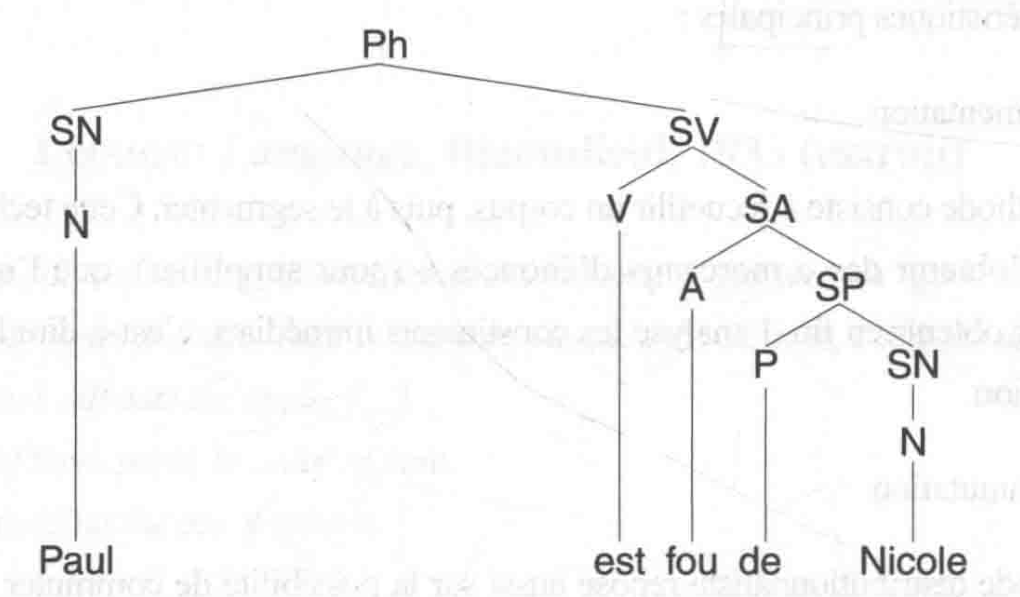
\includegraphics[width=.84\textwidth,height=.34\textheight,keepaspectratio]{assets/v17_sa.png}\end{center}

\minititle{4. Hiérarchie des constituants immédiats}

Si l’analyse distributionnelle consiste à définir l’environnement d’une unité du discours, elle suppose aussi une hiérarchie entre les constituants. Prenons un exemple :\par

\noindent\textbf{Ex :} Le vieux professeur donne un cours de syntaxe.\par

Par le biais de segmentations successives, les unités terminales (morphèmes) « vieux » et « professeur » sont appelés « constituants immédiats » de l’unité supérieure « vieux professeur », qui est un groupe nominal (GN).\par

Au niveau supérieur encore, le syntagme nominal (SN) « le vieux professeur » est constitué du GN et du déterminant « le », ainsi de suite : depuis les morphèmes isolés jusqu’à la phrase entière, chaque constituant s’emboîte dans un constituant de niveau supérieur, comme les briques d’une maison.\par



\origpage{441}{427}

\minititle{③ Les représentations graphiques}
Pour représenter cette analyse en constituants immédiats et donner à voir cette hiérarchie invisible entre constituants immédiats, les linguistes ont proposé différentes représentations graphiques. Ce qui suit devrait vous rappeler les stemmas des Tesnière.
\minititle{1. Les arborescences}
La représentation la plus employée est, sans aucun doute, celle de l’arbre syntaxique, appelé aussi indicateur syntagmatique. Sur le schéma ci-dessous, le syntagme apparaît bien comme l’unité syntaxique située entre la phrase et les constituants immédiats.
\begin{center}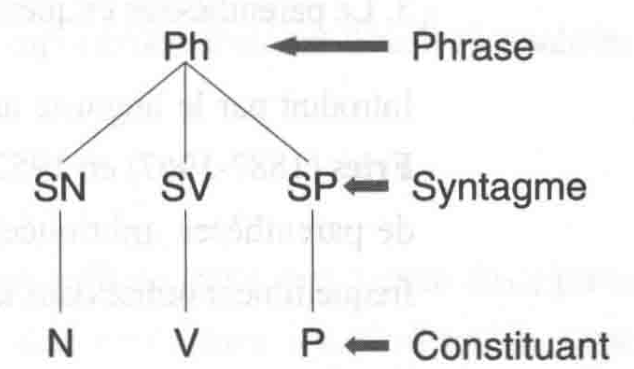
\includegraphics[width=.55\textwidth,height=.34\textheight,keepaspectratio]{assets/v17_schematic.png}\end{center}
Les arborescences représentent les différents constituants de la phrase, à l’image d’un arbre. En voici un autre exemple :
\begin{center}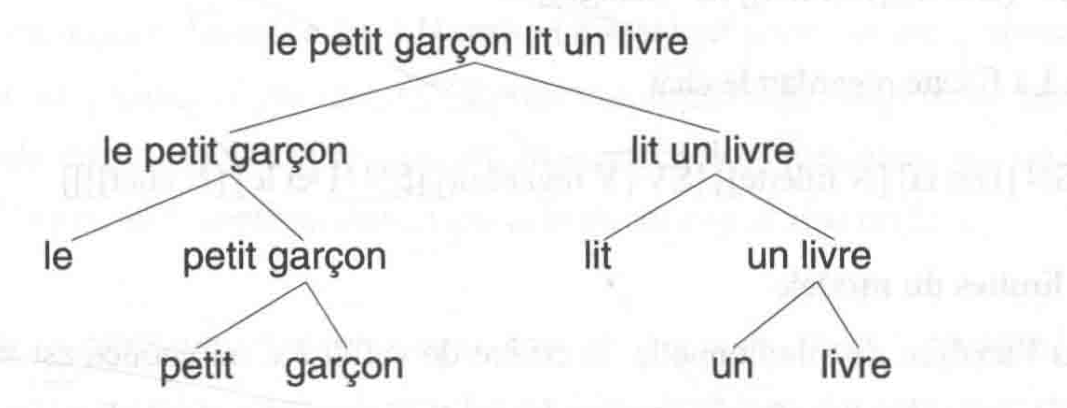
\includegraphics[width=.84\textwidth,height=.34\textheight,keepaspectratio]{assets/v17_boytree.png}\end{center}
\minititle{2. Les boîtes de Hockett}
Linguiste structuraliste américain, professeur de linguistique et d’anthropologie, \textbf{Charles Hockett} (1916-2000) a proposé en 1958 une représentation graphique de la structure de phrase sous la forme de boîtes à laquelle il a donné son nom. Dans les boîtes de Hockett, l’analyse progresse de la phrase (en bas de tableau) vers les constituants terminaux (situés en haut de tableau). La phrase est divisée en syntagmes, eux-mêmes segmentés en constituants immédiats. On procède ainsi jusqu’à obtenir des unités indivisibles : des morphèmes. En voici deux exemples :
\noindent\textbf{Ex :} Le grand chien blanc mangeait un os.
\begin{center}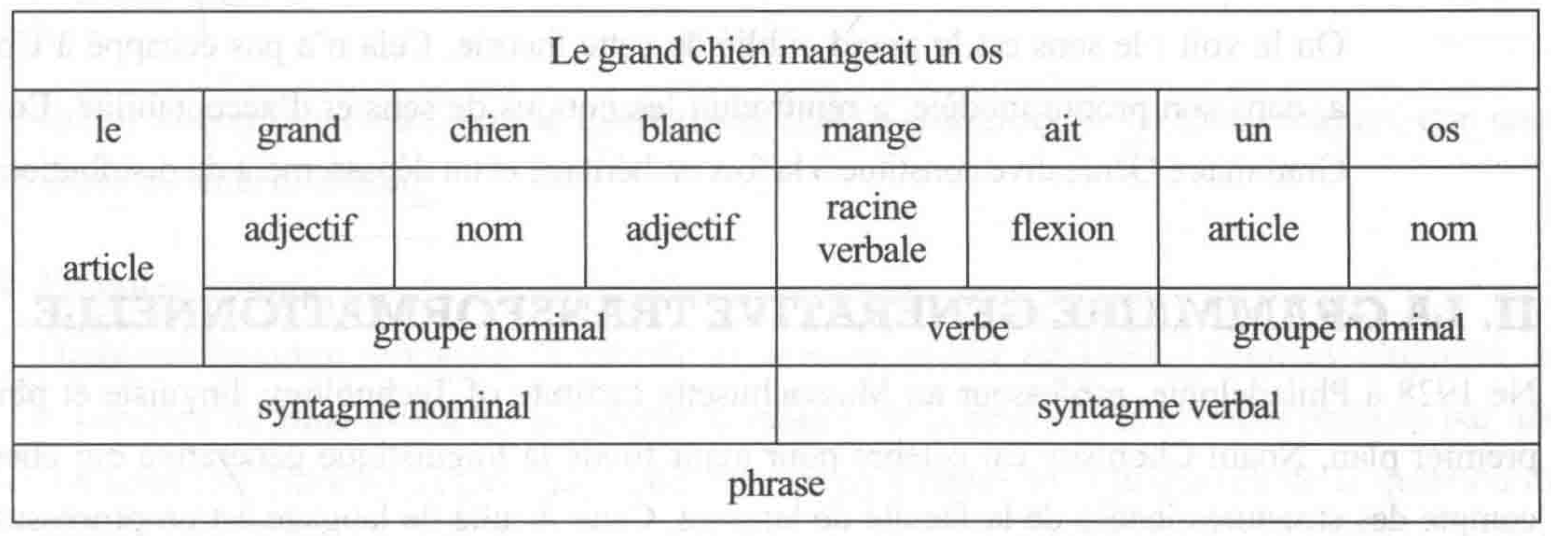
\includegraphics[width=.84\textwidth,height=.34\textheight,keepaspectratio]{assets/v17_hockett1.png}\end{center}
\noindent\textbf{Ex :} La fillette regardait le chat.

\origpage{442}{428}

\begin{center}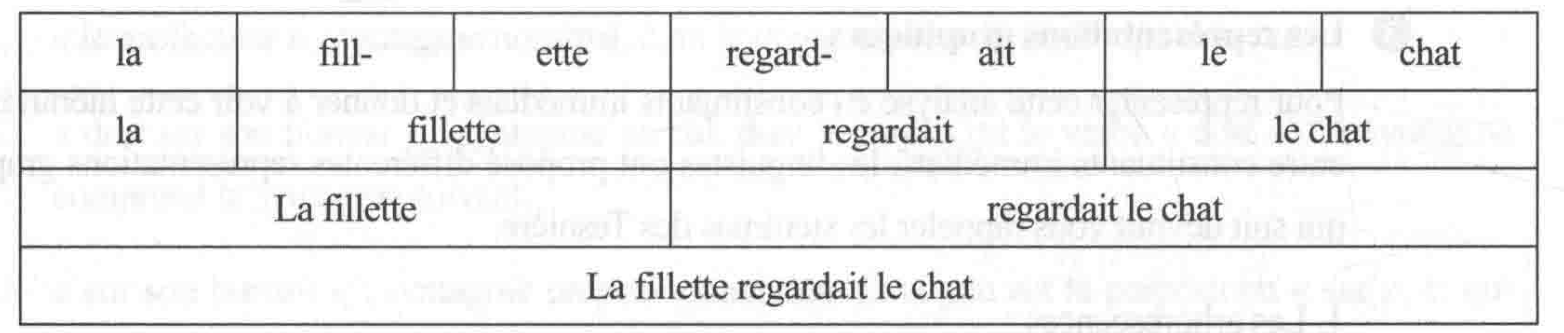
\includegraphics[width=.84\textwidth,height=.34\textheight,keepaspectratio]{assets/v17_hockett2.png}\end{center}

\minititle{3. Le parenthésage étiqueté}
Introduit par le linguiste américain et professeur à l’Université du Michigan Charles Carpenter Fries (1887-1967) en 1952, il consiste 4 représenter la structure syntaxique de la phrase au moyen de parenthéses imbriquées les unes dans les autres. De nos jours, le parenthésage étiqueté est fréquemment utilisé dans la tradition de Noam Chomsky. En voici deux exemples :\par

\noindent\textbf{Ex :} Le chien mange. [P [SN [Dét.le] [Nchien]] [SVmange]] Ex : La fillette regardait le chat.\par

[P [SN [Dé la] [N fillette]] [SV [V regardait] [SN [Dét le] [N chat]]]]\par

\minititle{④ Les limites du modèle}
Dans l’analyse distributionnelle, le critère de validité d’un énoncé est sa grammaticalité. Elle ne s’intéresse ni à son sens, ni à son acceptabilité. Prenons un exemple :\par

\noindent\textbf{Ex :} Un étudiant dort pendant le cours de linguistique.\par

« Étudiants » fait partie de la classe (du paradigme) des noms. En vertu de ce principe, et dans la perspective distributionnaliste, « étudiant » est donc commutable avec n’importe quel autre nom, par exemple « bureau » :\par

\noindent\textbf{Ex :} Un bureau dort pendant le cours de linguistique.\par

Dans la perspective distributionnaliste, cette phrase, malgré son asémantisme, sera jugée acceptable, car elle est grammaticale.\par

On le voit : le sens est le grand oublié de cette théorie. Cela n’a pas échappé à Chomsky, qui a, dans son propre modèle, a réintroduit les notions de sens et d’acceptabilité. En ce sens, sa\par

Grammaire Générative constitue à la fois un héritage et un dépassement du distributionnalisme.\par

\section{LA GRAMMAIRE GÉNÉRATIVE TRANSFORMATIONNELLE}

Né 1928 à Philadelphie, professeur au Massachusetts Institute of Technology, linguiste et philosophe de premier plan, Noam Chomsky est célèbre pour avoir fondé la linguistique générative qui cherche rendre compte des structures innées de la faculté de langage. Cette faculté de langage est un processus capable, à partir d’un nombre fini d'éléments (seulement 36 phonèmes en français\ednote{Le nombre de phonèmes du français dépend de la variété et de l’analyse retenues ; « 36 » ne constitue pas un inventaire universellement fixe. L’exemple peut être lu comme un ordre de grandeur pédagogique.}, rappelons-le), d’engendrer un nombre\par

\origpage{443}{429}

infini de phrases. Tournant majeur dans la manière d’étudier la structure des langues, la grammaire générative a fortement bousculé la linguistique traditionnelle et a influencé la psychologie, les neurosciences, la philosophie de l’esprit, et les sciences cognitives : c’est pour cela que l’on parle de « révolution chomskyenne ».\par

\subsection{La critique et dépassement du distributionnalisme}
Chomsky a développé sa théorie de la grammaire générative et transformationnelle dans les années 1950 en cherchant à dépasser les approches structuralistes, comportementalistes et distributionnalistes qui dominaient alors la scène linguistique.\par

\minititle{\textcircled{\scriptsize 1} Un triple rejet}

La linguistique chomskienne se distingue d’abord du structuralisme saussurien : toute description de la langue comme objet social ou historique est éliminée chez Chomsky, d’où son manque d’intérêt pour l’approche ethnologique des langues. Si la linguistique structurale a, selon Chomsky, correctement identifié un problème, à savoir comment faire émerger de la structure à partir de données linguistiques. Faisant écho à Harris et à Hockett pour qui une grammaire doit permettre d’engendrer les phrases d’une langue, Chomsky considère que l’approche purement descriptive du structuralisme, qui délaisse les mécanismes psychologiques créateurs du langage, doit être dépassée. C’est ce qu’il exprime dans Aspects of the theory of syntax (1965) :\par


\begin{lecture}{Extrait}
One of the qualities that all languages have in common is their ‘creative’ aspect. Thus an essential property of language is that it provides the means for expressing indefinitely many\par

| thoughts and for reacting appropriately in an indefinite range of new situations.
\end{lecture}
\par

Sa critique du Verbal Behavior de Skinner a remis en question l’approche comportementale de l’étude de l’esprit et du langage qui dominait dans les années 1950, et a amené à un retour aux positions « mentalistes » en linguistique, avec des références aux « idées innées » de Descartes : 
\begin{lecture}{Extrait}
Any interesting generative grammar will be dealing, for the most part, with mental processes that are far beyond the level of actual or even potential consciousness. [...] In the technical sense linguistic theory is mentalistic, since it is concerned with discovering a mental reality underlying actual behavior.
\end{lecture}
 Enfin, son opposition au modèle distributionnaliste a pris la forme de trois critiques, que nous allons détailler ci-dessous.\par

\minititle{\textcircled{\scriptsize 2} Première critique}
Dans son ouvrage fondateur, Syntactic Structures, publié en 1957, Chomsky s’oppose la conception de Bloomfield selon laquelle la langue est la somme des énoncés produits par une communauté. Chomsky pense que cette conception externe de la langue élude la question du rapport que le langage entretient avec l’esprit (mind) et le cerveau (brain) et laisse de côté la question de l’acquisition du langage. Quant à l’analyse en constituants immédiats, elle ne peut,\par

\origpage{444}{430}

selon lui, rendre compte du fait que des phrases à l’aspect formel semblable peuvent reposer sur des structures tout à fait différentes. Prenons un exemple :\par

\noindent\textbf{Ex :} L'enfant a été retrouvé par un malheureux clochard. L'enfant a été retrouvé par un heureux hasard.\par

L'analyse distributionnelle montre que les deux phrases ont une même structure : syntagme nominal, syntagme verbal et syntagme prépositionnel. Leur représentation sur un arbre syntaxique ou dans une boite de Hockett serait identique. Or, cette ressemblance n’est que superficielle. En effet, la première phrase peut être transformée à la voix active : Ex : Un malheureux clochard a retrouvé l’enfant.\par

Mais la transformation active n’est pas possible pour la seconde : Ex : * Un heureux hasard a retrouvé l’enfant.\par

L’analyse distributionnelle, pour Chomsky, ne permet pas de montrer la différence structurelle profonde qui existe entre ces deux énoncés.\par

\minititle{\textcircled{\scriptsize 3} Deuxième critique}
Corollaire inversé de la première critique, Chomsky note également qu’il n’est pas possible, dans le cadre de l’analyse en constituants immédiats, de montrer que des énoncés en apparence différents entretiennent en fait une certaine relation fondamentale :\par

\noindent\textbf{Ex :} Le chat mange la souris. /La souris est mangée par le chat.\par

Paul viendra. /Est-ce que Paul viendra ?\par

\minititle{\textcircled{\scriptsize 4} Troisième critique}
Enfin, le distributionnaliste étant asémantique, il ne se préoccupe pas du problème de l’ambiguïté syntaxique, lorsque plusieurs structures syntaxiques sont possibles pour un même énoncé, mais avec un sens complètement différent. En voici quelques exemples :\par

\noindent\textbf{Ex :} Le cuisinier sale la note.\par

\noindent\textbf{Ex :} Cet artiste peint la nuit.\par

\begin{center}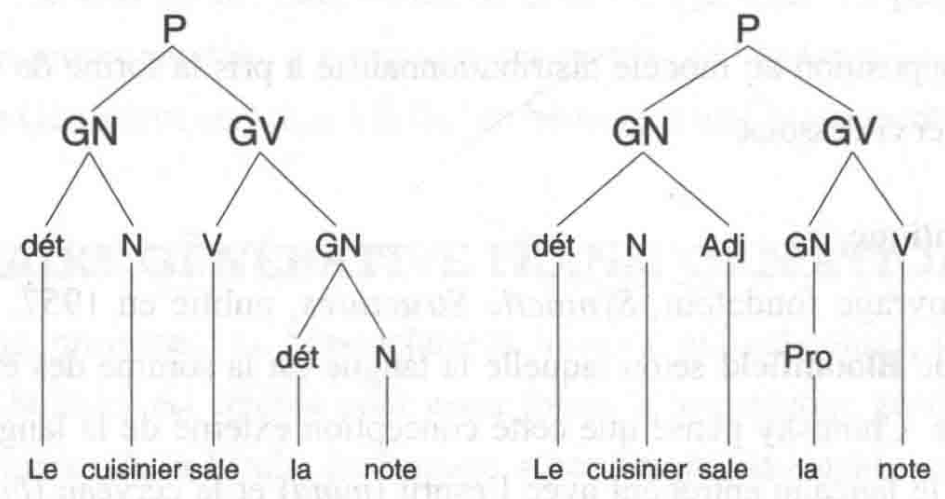
\includegraphics[width=.84\textwidth,height=.29\textheight,keepaspectratio]{assets/v17_ambiguity.png}\end{center}

\origpage{445}{431}

\begin{center}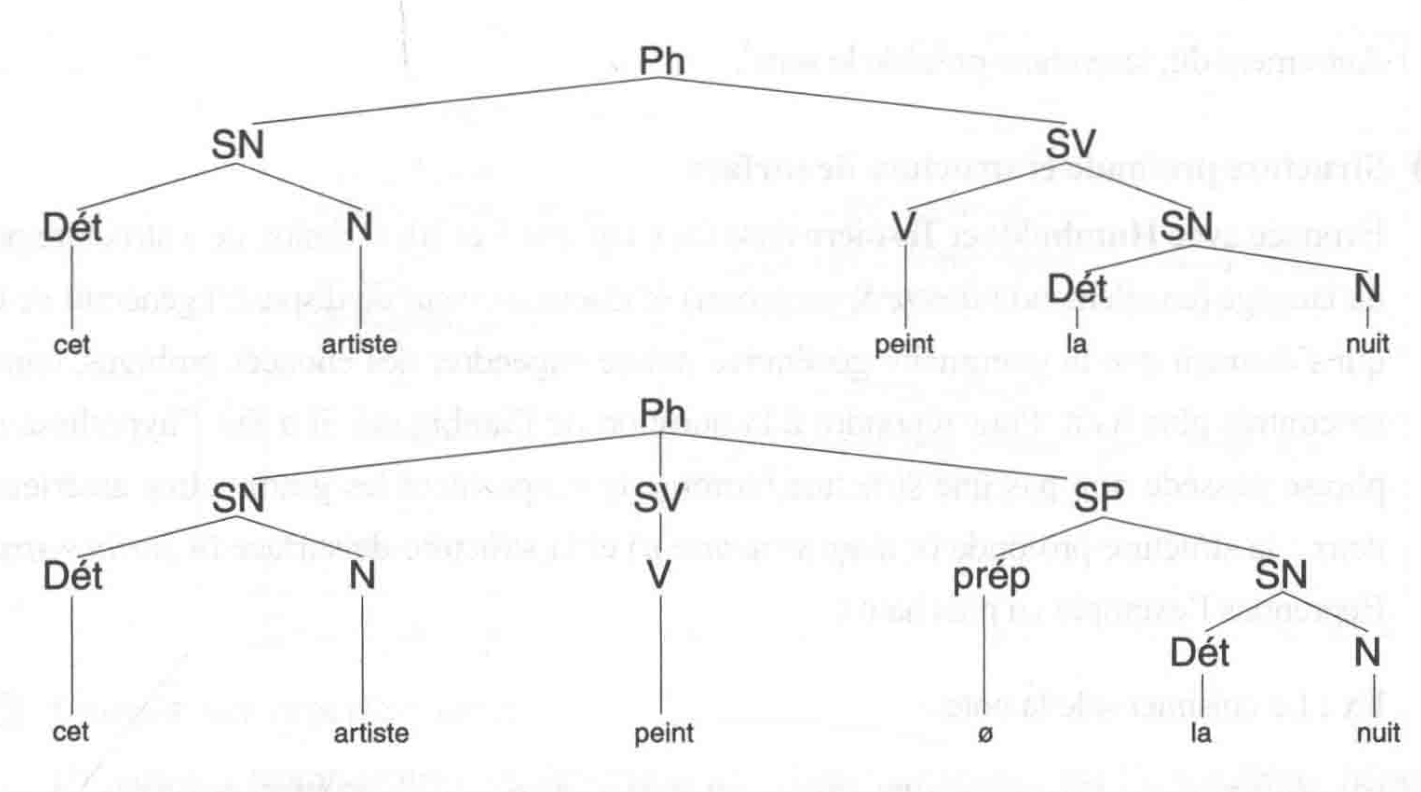
\includegraphics[width=.84\textwidth,height=.34\textheight,keepaspectratio]{assets/v17_artist.png}\end{center}

L’ambiguité peut être syntaxique, mais aussi sémantique, basée alors sur la polysémie, comme dans l’exemple ci-dessous :\par

\noindent\textbf{Ex :} Il s’est rendu au tribunal international de La Haye.\par

Malgré les interprétations différentes (« 他去了海牙法庭 » ou « 他去海牙法庭自首 »), l’analyse en composants immédiats de ces deux énoncés sera identique. Pour Chomsky, les ambiguïtés ne peuvent être dissipées dans le cadre de l’analyse distributionnelle.\par

\subsection{La Théorie Standard}
Après les critiques est venu le temps des propositions. Dans Aspects of the theory of syntax (1965), Chomsky a établi un nouveau type de grammaire. Cette grammaire est dite générative, conçue comme un mécanisme qui engendre les phrases d’une langue.\par

\minititle{\textcircled{\scriptsize 1} Une approche modulaire}
Le premier modèle génératif de Chomsky est modulaire : c’est un système de sous-systèmes (modules) indépendants et interagissants. Dans cette optique générative, la langue est considérée comme un macrosystème structurel composé de microsystèmes ayant leur propre structure. Ces modules sont au nombre de trois :\par

la syntaxe, qui donne une structure à la phrase. © la phonologie, qui donne une forme phonétique à la phrase. © la sémantique, qui donne une interprétation à la phrase.\par

Pour Chomsky, la partie centrale de cette grammaire est la syntaxe, et deux autres modules ne peuvent pas occuper cette place centrale. En effet, pour que la phonologie puisse donner une forme phonétique aux phrases, il faut que ces phrases soient déjà formées. Et pour que la sémantique puisse donner aux phrases une interprétation, il faut que l’on connaisse leur structure : c’est ce que nous venons de voir dans le cas des phrases ambiguës. C’est la structure qui donne le sens.\par



\origpage{446}{432}

Autrement dit, la syntaxe précède le sens\origfoot{3}{Nous verrons dans le dernier chapitre que ce modèle chomskyen, centré sur la syntaxe, a soulevé à l’époque récente un certain nombre de critiques.}.\par

\minititle{\textcircled{\scriptsize 2} Structure profonde et structure de surface}

Évoquée avec Humboldt et Tesniére dans les chapitres 5 et 10, la notion de « structure profonde » du langage (en allemand : Innere Sprachform) se trouve au cœur du dispositif génératif de Chomsky qui s’étonnait que la grammaire générative puisse engendrer des énoncés ambigus, comme ceux rencontrés plus haut. Pour répondre à la question de l’ambiguïté, il a fait l'hypothèse que toute phrase possède non pas une structure, comme le supposaient les grammaires antérieures, mais deux : la structure profonde (« deep structure ») et la structure de surface (« surface structure »). Reprenons l’exemple vu plus haut :\par

\noindent\textbf{Ex :} Le cuisinier sale la note.\par

Si cette phrase a deux sens différents (« 厨子漫天要价 » ou « 脏厨子给她打分 »), c’est parce qu’elle a deux structures profondes (SP-1 et SP-2) distinctes. Dans le cas des phrases non ambigués, à chaque structure profonde correspond une structure de surface qui lui est propre. Mais dans notre exemple, les deux structures profondes distinctes possèdent une structure de surface (SS-1 et SS-2) identique. Pour Chomsky, c’est la distinction entre la structure de surface d’une phrase et sa structure profonde qui permet d’expliquer l’existence de phrases ambiguës.\par

De la même façon, c’est la distinction entre la structure de surface et sa structure profonde qui permet d’expliquer pourquoi deux phrases différentes sur le plan phonologique ont le même sens. Reprenons encore un exemple vu plus haut :\par

\noindent\textbf{Ex :} Le chat mange la souris. / La souris est mangée par le chat.\par

Pour Chomsky, et à l’inverse du premier exemple, ces deux phrases ont deux structures de surface différentes, mais ont une structure profonde totalement identique, la seconde phrase étant la « transformation » passive de la première, illustrée dans le schéma ci-dessous sur lequel vous retrouverez les trois modules : syntaxe, phonologie, et sémantique. J’attire votre attention sur le fait que la structure profonde est reliée au module sémantique : la structure profonde, on l’a vu, détermine (en partie) le sens d’un énoncé. Quant aux règles de réécriture du module syntaxique, elles seront expliquées un peu plus bas.\par

\origpage{447}{433}

\begin{center}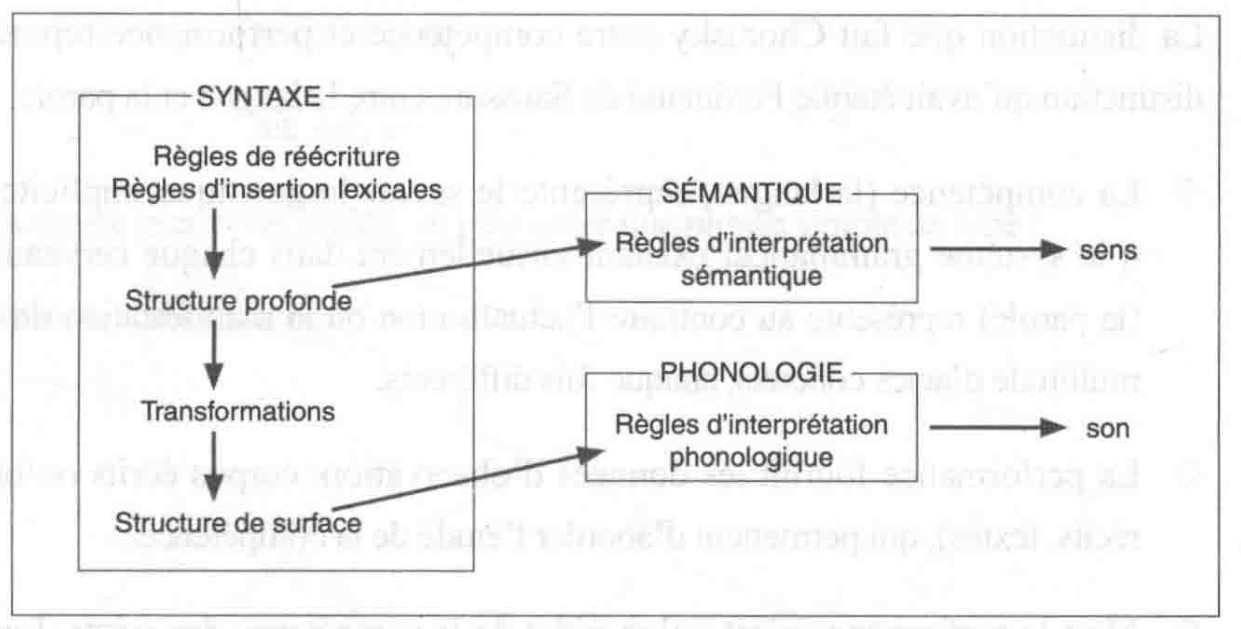
\includegraphics[width=.84\textwidth,height=.34\textheight,keepaspectratio]{assets/v17_standard.png}\end{center}
\minititle{③ Compétence et performance}
Un autre concept central de \emph{Aspects of the theory of syntax} est l’opposition théorique entre \emph{competence et performance}, réinterprétation par Chomsky de l’opposition saussurienne entre langue et parole. Par compétence, Chomsky entend la connaissance que le locuteur-auditeur a de sa langue, par opposition à la performance, c’est-à-dire l’emploi effectif de la langue dans des situations concrètes :
\begin{lecture}{Extrait}
We thus make a fundamental distinction between competence (the speaker-hearer’s knowledge of his language) and performance (the actual use of language in concrete situations).
\end{lecture}
Pour Chomsky, la tâche du linguiste ne consiste pas à décrire la performance et les énoncés déjà produits mais à prédire la compétence, c’est-à-dire la construction de ces énoncés :
\begin{lecture}{Extrait}
Hence, in the technical sense, linguistic theory is mentalistic, since it is concerned with discovering a mental reality underlying actual behavior. Observed use of language may provide evidence as to the nature of this mental reality, but surely cannot constitute the actual subject matter of linguistics, if this is to be a serious discipline.
\end{lecture}
Pour le locuteur-auditeur, la compétence (connaissance de la langue) est double : il s’agit bien sûr de la capacité de \emph{construire} des énoncés, mais aussi de les \emph{comprendre} et de \emph{reconnaître} s’ils sont (ou ne sont pas) grammaticaux, sémantiques, ambigus, etc. C’est ce qu’explique \textbf{Nicolas Ruwet} (1933-2001), connu pour son \emph{Introduction à la grammaire générative} (1967) :
\begin{lecture}{Extrait}
Il apparaît immédiatement que le fait central, dont la linguistique synchronique a à s’occuper, est le suivant : tout sujet adulte parlant une langue donnée est, à tout moment, capable d’émettre spontanément, ou de percevoir et de comprendre, un nombre indéfini de phrases que, pour la plupart, il n’a jamais prononcées ni entendues auparavant Tout sujet parlant possède donc certaines aptitudes très spéciales, qu’on peut appeler sa compétence linguistique, et qu’il a acquises, dans son enfance, au cours de la brève période d’apprentissage de sa langue.
\end{lecture}

\origpage{448}{434}

La distinction que fait Chomsky entre compétence et performance reprend en la précisant la distinction qu’avait établie Ferdinand de Saussure entre la langue et la parole.\par

La compétence (la langue) représente le savoir linguistique implicite des sujets parlants, « le système grammatical existant virtuellement dans chaque cerveau »\origfoot{4}{Saussure (Ferdinand de). \emph{Cours de linguistique générale}, Paris, Payot, 1916, 30p.}. La performance (la parole) représente au contraire l’actualisation ou la manifestation de ce système dans une multitude d’actes concrets, chaque fois différents.\par

La performance fournit les données d’observation, corpus écrits ou oraux (conversations,\par

récits, textes), qui permettent d’aborder l’étude de la compétence.\par

Mais la performance n’est qu’un reflet de la compétence des sujets. Les actes de parole des sujets ne dépendent pas uniquement de leur compétence linguistique : ils varient en fonction d’un grand nombre d’autres facteurs tels que la mémoire, l’attention, la motivation, l’émotivité, etc., qui ne relèvent pas de la linguistique.\par

Notez enfin que pour Chomsky, la compétence et les structures profondes résident dans l’esprit : elles sont innées et font partie de l’héritage biologique de chacun. Nous reviendrons sur cela de façon détaillée dans le prochain chapitre, Biolinguistique et psycholinguistique.\par

\minititle{\textcircled{\scriptsize 4} Les règles de réécriture (rewriting rules)}

Le processus génératif repose sur un ensemble de règles en nombre très limité, les rewritings rules («règles de réécriture »), utilisées pour créer des syntagmes qui, à leur tour, vont créer des énoncés. Si les distributionnalistes partaient d’un énoncé déjà constitué pour le décomposer en syntagmes puis en constituants immédiats, la démarche de Chomsky est inverse : il part des constituants immédiats pour créer des syntagmes puis une infinité de phrases grammaticales, en suivant des règles d’assemblages — les règles de réécriture, appelées aussi règles syntagmatiques, et dont la connaissance est innée.\par

Dans les règles de réécriture présentées ci-dessous. « S » désigne la phrase (sentence), « NP » le syntagme nominal (nominal phrase), « VP » le syntagme verbal (verbal phrase), « Det » le déterminant, « N » le substantif (noun), et « Aux » l’auxiliaire.\par

\begin{align*}
(1)\quad\mathrm{S}&\longrightarrow\mathrm{NP+VP}\\
(2)\quad\mathrm{VP}&\longrightarrow\mathrm{Verb+NP}\\
(3)\quad\mathrm{NP}&\longrightarrow\mathrm{Det+N}\\
(4)\quad\mathrm{Verb}&\longrightarrow\mathrm{Aux+V}\\
(5)\quad\mathrm{Det}&\longrightarrow\text{the, a, etc.}\\
(6)\quad\mathrm{N}&\longrightarrow\text{man, ball, etc.}
\end{align*}

\origpage{449}{435}

\begin{align*}
(7)\quad\mathrm{Aux}&\longrightarrow\text{will, can, etc.}\\
(8)\quad\mathrm{V}&\longrightarrow\text{hit, see, etc.}
\end{align*}
Avec les quatre premières règles, on peut créer une phrase simple de type :
\noindent\textbf{Ex :} \emph{The man will hit the ball.}
\begin{center}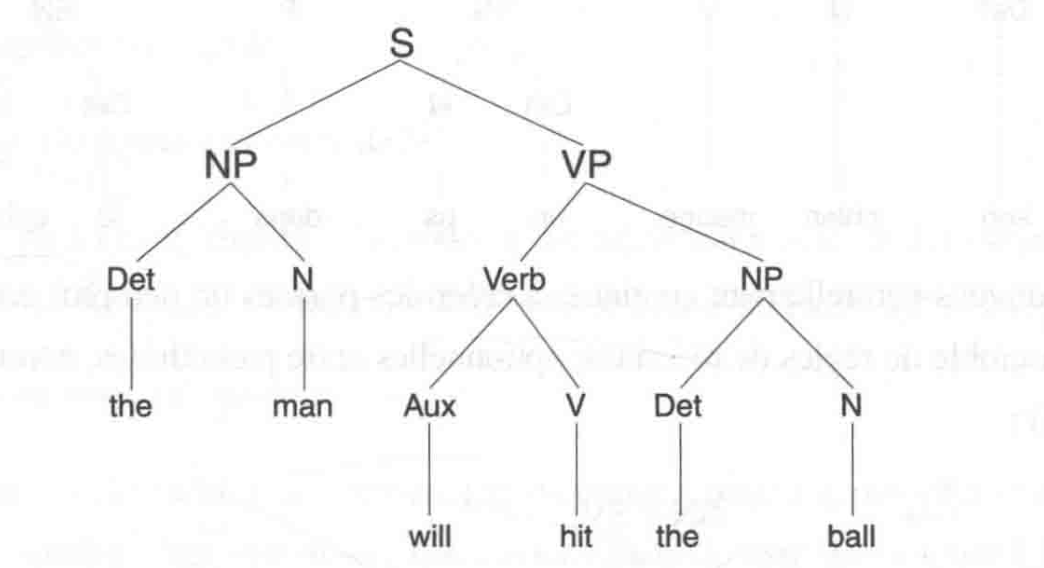
\includegraphics[width=.84\textwidth,height=.34\textheight,keepaspectratio]{assets/v17_mantree.png}\end{center}
Puis, à l’aide des très nombreux déterminants (5), noms (6), auxiliaires (7) et verbes (8), que nous pouvons entrer comme \emph{input} dans cette « machine fabriqué des énoncés », nous obtiendrons une infinité de nouvelles phrases :
\noindent\textbf{Ex :} \emph{The boy will read the book.}
\begin{center}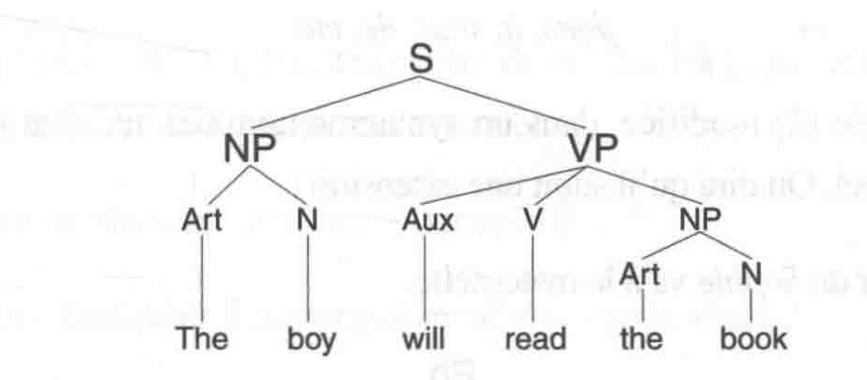
\includegraphics[width=.84\textwidth,height=.34\textheight,keepaspectratio]{assets/v17_boyread.png}\end{center}
Pour complexifier un peu les énoncés produits, on peut rajouter une règle de réécriture pour créer des syntagmes prépositionnels (SP) à l’aide de prépositions (P), comme ci-dessous, avec les règles (4) et (5) :
\begin{align*}
(1)\quad\mathrm{Ph}&\longrightarrow\mathrm{SN+SV}\\
(2)\quad\mathrm{SN}&\longrightarrow\text{Dét}+\mathrm{N}\\
(3)\quad\mathrm{SV}&\longrightarrow\mathrm{V+SN}\\
(4)\quad\mathrm{SP}&\longrightarrow\mathrm{P+SN}\\
(5)\quad\mathrm{P}&\longrightarrow\text{dans, à, sous, de, etc.}
\end{align*}
On pourra alors fabriquer une infinité de phrases sur le modèle suivant :
\noindent\textbf{Ex :} Son chien mange un os \emph{dans la cuisine}.

\origpage{450}{436}

L’arborescence ci-dessous nous permet de visualiser les règles de réécriture, et le nouveau syntagme prépositionnel (SP) créé à l’aide des règles (4) et (5):
\begin{center}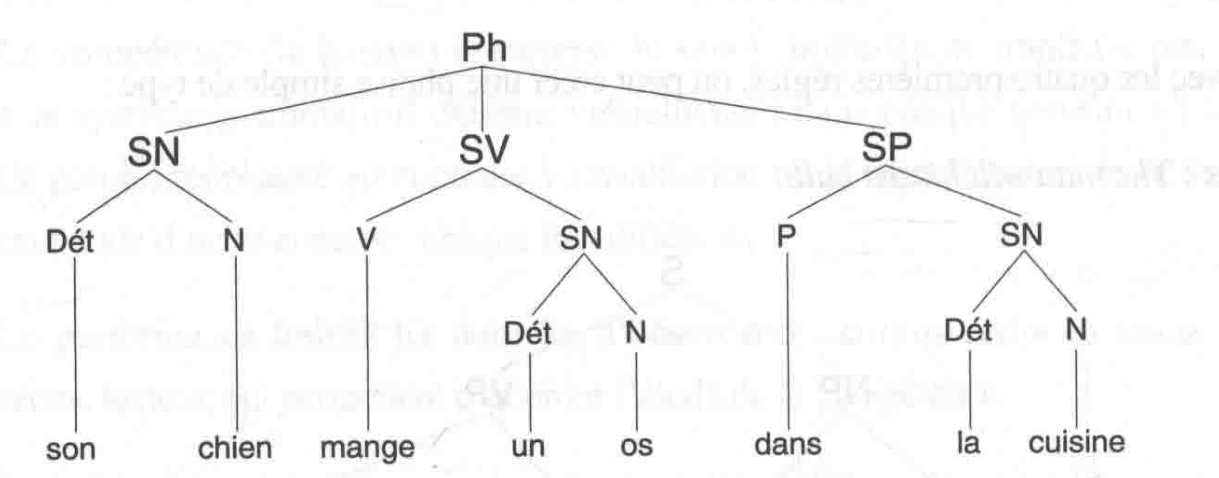
\includegraphics[width=.84\textwidth,height=.34\textheight,keepaspectratio]{assets/v17_dogtree.png}\end{center}
Nous pouvons naturellement continuer à créer des phrases un peu plus complexes en utilisant un sous-ensemble de règles de réécriture optionnelles entre parenthèses, comme par exemple dans la règle (2) :
\begin{align*}
(1)\quad\mathrm{Ph}&\longrightarrow\mathrm{SN+SV}\\
(2)\quad\mathrm{SN}&\longrightarrow\text{Dét}+\mathrm{N+(SP)}\\
(3)\quad\mathrm{SV}&\longrightarrow\mathrm{V+SP}\\
(4)\quad\mathrm{SP}&\longrightarrow\mathrm{P+SN}\\
(5)\quad\mathrm{P}&\longrightarrow\text{dans, à, sous, de, etc.}
\end{align*}
Selon la règle (2) modifiée, dans un syntagme nominal, un nom \emph{peut} être suivi d’un syntagme prépositionnel. On dira qu’il subit une extension :
\begin{itemize}\item La sœur de \emph{Sophie} va à la maternelle.\end{itemize}
\begin{center}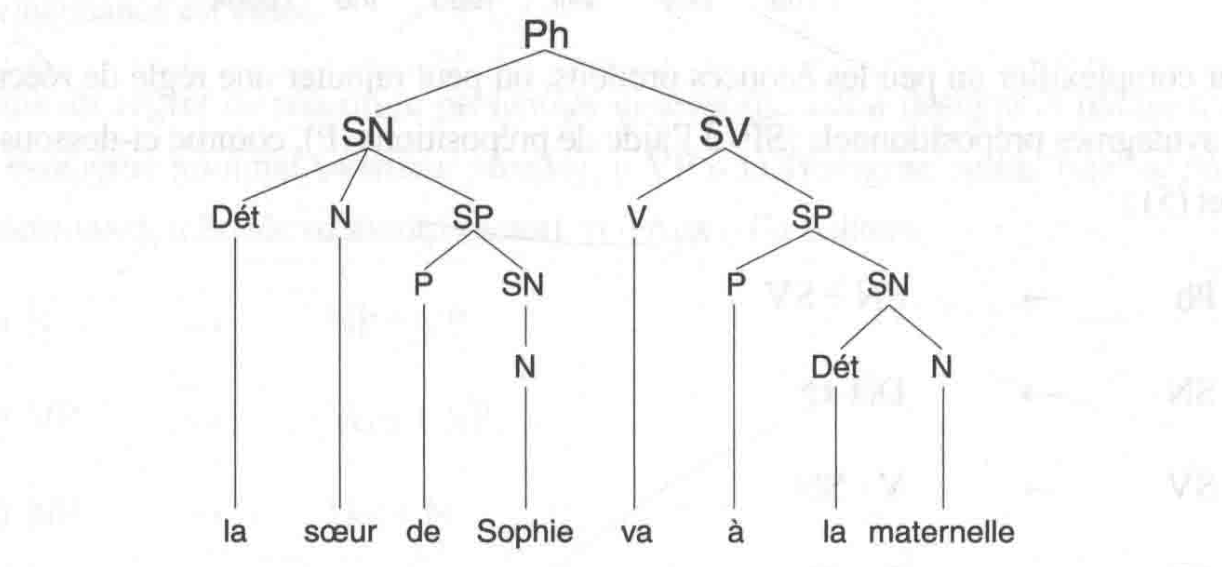
\includegraphics[width=.84\textwidth,height=.34\textheight,keepaspectratio]{assets/v17_sophietree.png}\end{center}
\minititle{⑤ Les règles transformationnelles}
En faisant l’hypothèse que la compétence, la structure profonde et les règles de réécriture résident dans notre esprit, Chomsky a ajouté une dimension mentaliste à la perspective mécaniste des distributionnalistes. C’est à la fois un progrès et une rupture considérables, mais la première version de cette grammaire à capacité générative a deux défauts :

\origpage{451}{437}

D'une part, elle donne des descriptions semblables de phrases de sens différent : Ex : Pierre envoie des fleurs à Marie.\par

Pierre envoie des fleurs à Rome. © D'autre part, elle donne des descriptions différentes de phrases de sens semblable : Ex : Le professeur est malade\par

Est-ce que le professeur est malade ?\par

Pour répondre à ces critiques, Chomsky a introduit dans son modèle standard la notion de transformation. Dès lors, sa grammaire va devenir générative et transformationnelle.\par

\minititle{1. Les transformations syntaxiques}

La notion de transformation ne vous est pas inconnue : nous l’avons déjà rencontrée, souvenez- vous, chez Tesnière. Pour être précis, nous avions parlé de translation. Chez Chomsky, le passage de la structure profonde abstraite à la structure de surface se fait à travers des transformations syntaxiques qui permettent de supprimer, d’ajouter ou de déplacer un ou plusieurs éléments dans la phrase. Prenons quelques exemples :\par

\noindent\textbf{Ex :} Tu viens / Est-ce que tu viens ? / Viens-tu ? / Viens !\par

Pour obtenir une phrase interrogative (structure de surface) à partir d’une phrase affirmative (structure profonde) il faudra transformer cette dernière :\par

Soit en déplaçant un élément : tu viens — viens-tu ?\par

soit en ajoutant un marqueur d’interrogation : Est-ce que tu viens ?\par

À l'impératif, la transformation se fera à travers la suppression d’un élément (le sujet). Ex : Will the boy leave ?\par

La phrase interrogative ci-dessus est le résultat de la transformation, dans la structure profonde, de la phrase affirmative « the boy will leave ».\par


\begin{center}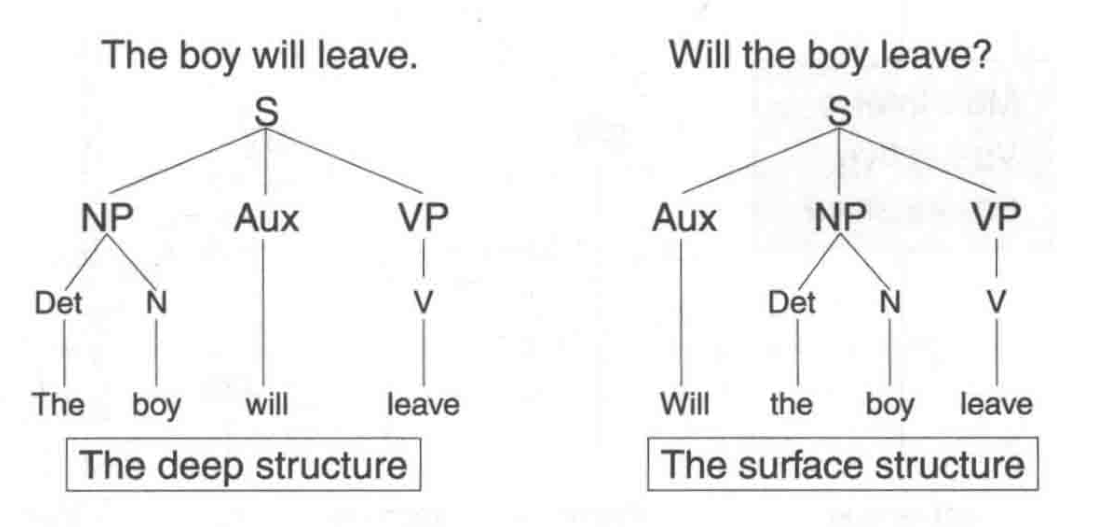
\includegraphics[width=.84\textwidth,height=.34\textheight,keepaspectratio]{assets/v17_deepsurface.png}\end{center}

\origpage{452}{438}

\minititle{2. Les différents types de transformations}
Dans sa globalité, la phrase, représentée par le signe $\Sigma$ (sigma) est constituée d’un type (T) et d’un matériau (Ph).
\begin{itemize}
\item Le type (T) comprend le mode (indicatif, interrogatif, impératif), la voix (active, passive), et la polarité (positive, négative).
\item Le matériau correspond à la phrase de base (\emph{kernel sentence}) en structure profonde qui pourra faire l’objet de transformations syntaxiques.
\end{itemize}
La phrase globale peut donc être représentée ainsi :
\begin{center}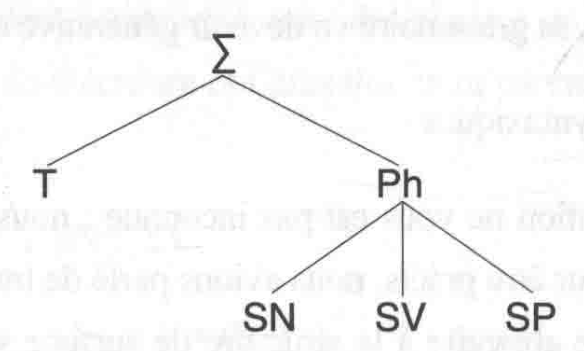
\includegraphics[width=.5\textwidth,height=.34\textheight,keepaspectratio]{assets/v17_sigma.png}\end{center}
Les transformations portent sur le type (T), autrement dit sur le mode (Mo), les polarités (Po) et la voix (Vo). Prenons comme matériau l’exemple suivant :
\noindent\textbf{Ex :} Pierre apprécie ce livre.

Dans la structure profonde, cette phrase de base pourra faire l’objet des transformations suivantes :
\minititle{1) Transformation interrogative}
\noindent\textbf{Ex :} Est-ce que Pierre apprécie ce livre ?

À droite de l’arborescence se trouve la phrase de base (Ph). À gauche, le type de phrase (T) indique la transformation en mode (Mo) interrogatif :
\begin{center}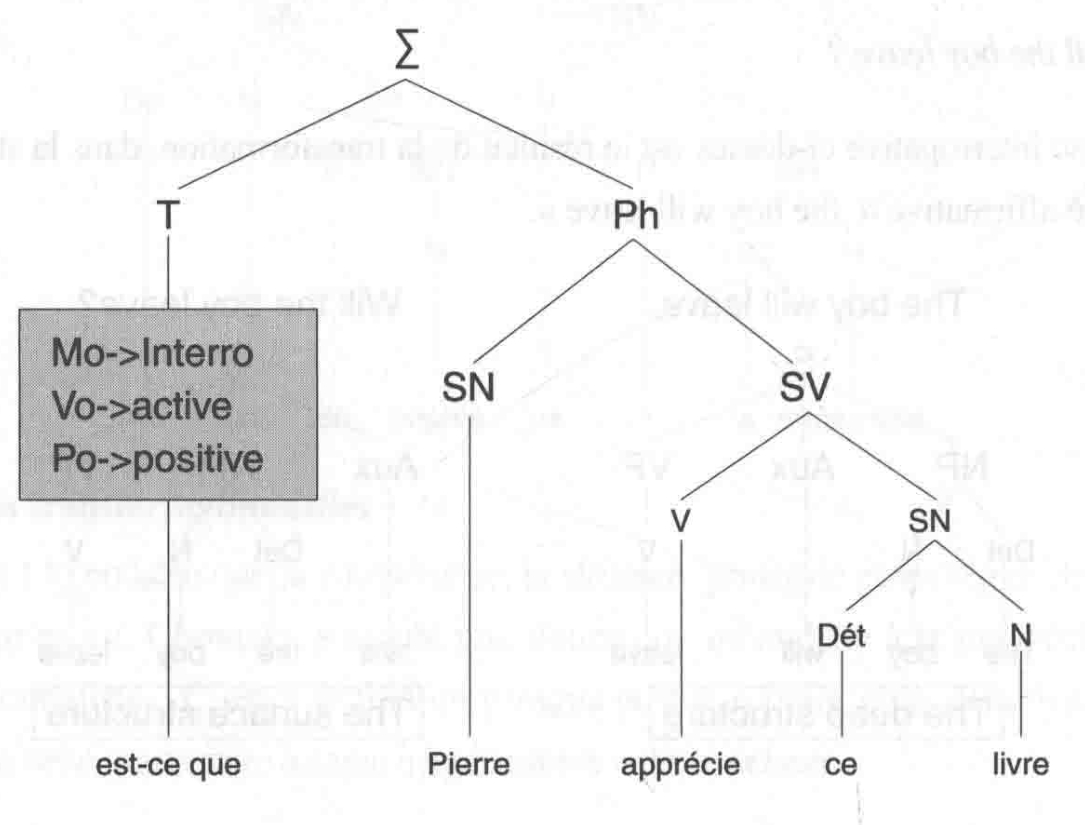
\includegraphics[width=.84\textwidth,height=.34\textheight,keepaspectratio]{assets/v17_interrogative.png}\end{center}

\origpage{453}{439}

\minititle{2) Transformation passive}
\noindent\textbf{Ex :} Ce livre est apprécié par Pierre.

Le type de phrase (T) indique la transformation de voix (Vo) passive :
\begin{center}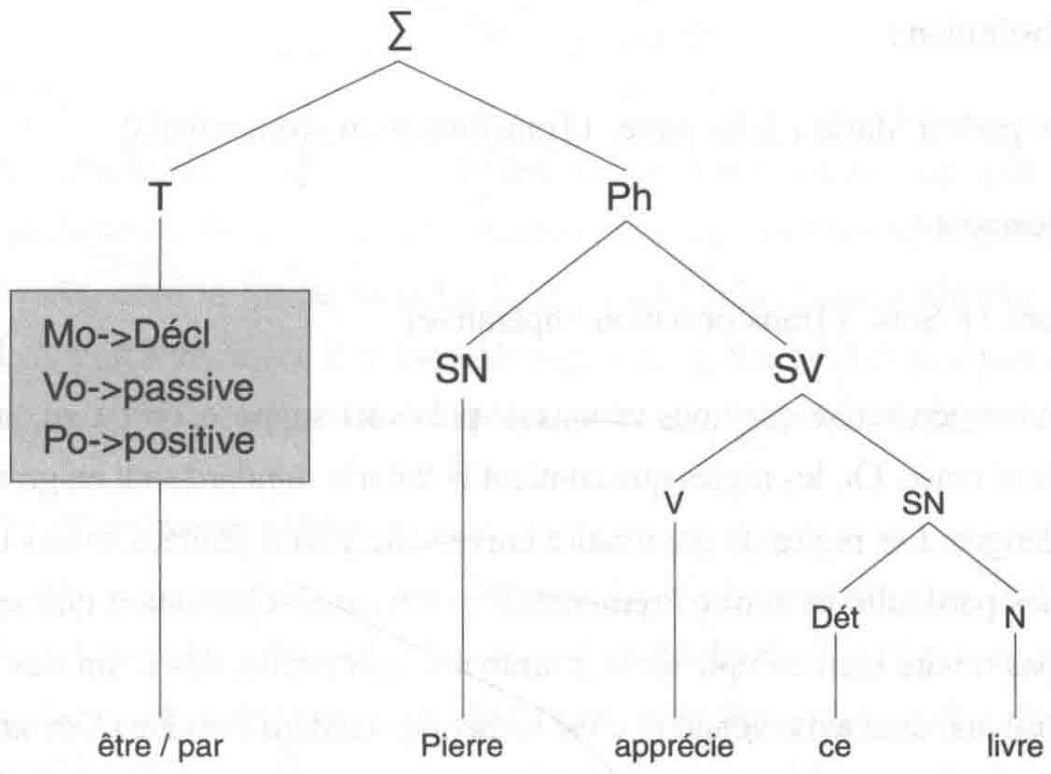
\includegraphics[width=.84\textwidth,height=.34\textheight,keepaspectratio]{assets/v17_passive.png}\end{center}
\minititle{3) Transformation négative}
\noindent\textbf{Ex :} Pierre n’apprécie pas ce livre.

Le type de phrase (T) indique la transformation de la polarité (Po) :
\begin{center}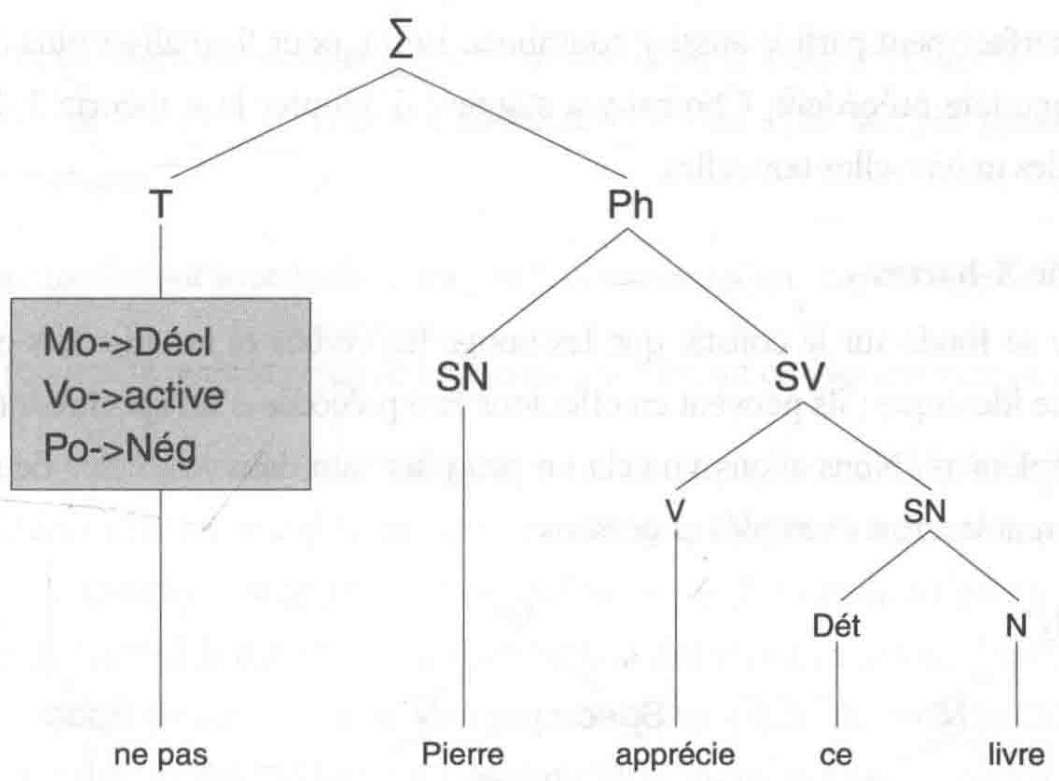
\includegraphics[width=.84\textwidth,height=.34\textheight,keepaspectratio]{assets/v17_negative.png}\end{center}
\minititle{3. Les procédés morphosyntaxiques de transformation}
Les transformations ci-dessus sont les résultats manipulations morphosyntaxiques, dont les plus fréquentes sont :
\minititle{L’addition :}

\origpage{454}{440}

\noindent\textbf{Ex :} Je pars. / Je ne pars pas. (Transformation négative)\par

\minititle{Le déplacement :}
\noindent\textbf{Ex :} Tu viens. / Viens-tu ? (Transformation interrogative)\par

\minititle{La substitution :}
\noindent\textbf{Ex :} Pierre parle à Marie. / Il lui parle. (Transformation pronominale) \minititle{L’effacement :}\par

\noindent\textbf{Ex :} Tu sors. /\#Sors. (Transformation impérative)\par

La grammaire générative que nous venons de présenter suppose, on l’a vu, une faculté de langage universelle et innée. Or, les règles que contient la théorie standard sont en grande partie spécifiques à chaque langue. Les règles de grammaire universelle y sont limitées, tandis que les règles propres aux langues particulières sont extrêmement nombreuses. Constatant que sa théorie standard ne semblait pas rendre bien compte de la grammaire universelle, dès la fin des années 60, Chomsky en a proposé une deuxième version : c’est la théorie standard étendue (Extended Standard Theory).\par

\subsection{La Théorie Standard Étendue}
Avec la théorie standard étendue, Chomsky met à jour de nouvelles règles universelles et propose un modèle dans lequel la grammaire universelle est plus importante que les règles des langues particulières. Ensuite, la structure profonde n’est plus seule à déterminer le sens de la phrase : la structure de surface peut parfois aussi y contribuer. Enfin, pour formaliser plus de règles universelles que dans le modèle précédent, Chomsky a suggéré d’adopter la « théorie X-barres », une de ces nouvelles règles universelles nouvelles.\par

\minititle{\textcircled{\scriptsize 1} La théorie X-barres}
Chomsky se fonde sur le constat que les noms, les verbes et les adjectifs ont un comportement syntaxique identique : ils peuvent en effet tous être précédés d’un spécifieur (déterminant) et suivi d’un complément. Nous avons vu cela un peu plus haut dans les règles de réécriture, et c’est ce que montrent les trois exemples ci-dessous :\par

\begin{center}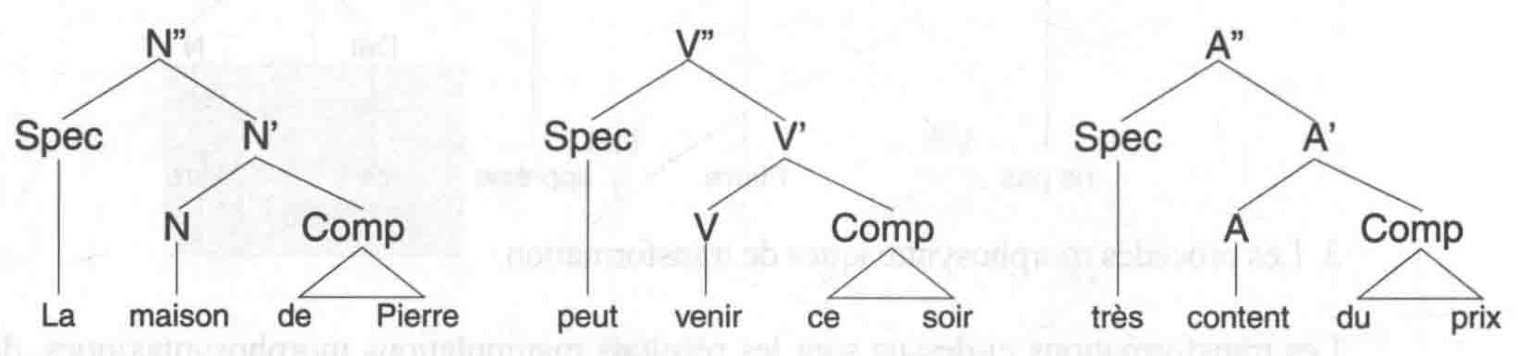
\includegraphics[width=.84\textwidth,height=.34\textheight,keepaspectratio]{assets/v17_xexamples.png}\end{center}

Selon le modèle standard, ces trois structures de surface sont engendrées par trois séries de règles de réécriture, c’est-à-dire une série pour chaque structure. Mais, puisqu’au fond elles sont identiques, Chomsky propose de n’adopter qu’une seule série de règles de réécriture pour obtenir une structure unique. Dans cette structure, le nom (N), le verbe (V) ou l’adjectif (A) sont remplacés\par



\origpage{455}{441}

par un seul et unique X, comme suit :\par

\begin{center}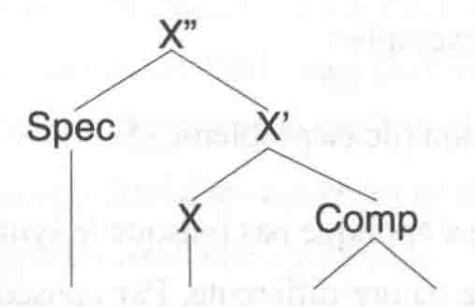
\includegraphics[width=.84\textwidth,height=.34\textheight,keepaspectratio]{assets/v17_xgeneral.png}\end{center}

C'est cette généralisation de trois schémas en un que Chomsky appelle « théorie X-barres ». Cette hypothèse de l’existence d’un schéma unique pour les syntagmes nominaux, verbaux et adjectivaux, dont la forme dans les langues particulières peut différer mais dont le principe universel conduit à diminuer le nombre de règles particulières et donc à rendre mieux compte de la grammaire universelle : c’était un des objectifs de cette la théorie étendue.\par

\minititle{\textcircled{\scriptsize 2} Conditions on Transformations}

Toujours dans le même esprit, afin de limiter les règles particulières et d’augmenter les règles universelles, Chomsky a formulé une nouvelle hypothèse : l’application des transformations est soumise à des conditions, et ces conditions sont, elles aussi, universelles. Prenons l’exemple de la transformation pronominale évoquée plus haut. Il est possible, nous le savons, de transformer un syntagme nominal à l’aide du pronom « en », comme ci-dessous :\par

\noindent\textbf{Ex :} Pierre est fier de son travail. — Pierre en est fier. Mon ami veut de la bière — mon ami en veut.\par

Comme la grammaire chomskyenne universelle, il peut sembler étonnant que la même transformation (« de » + « syntagme nominal » — « en ») ne soit pas possible dans certains cas, comme ci-dessous :\par

\noindent\textbf{Ex :} Pierre médite sur le sens de sa vie. — * Pierre en médite sur le sens. Pierre viendra avec la sœur de sa femme. — * Pierre en viendra avec la sœur.\par

Dans le cadre de la théorie standard, pour rendre compte de cette impossibilité, il était nécessaire de mettre au point un grand nombre de règles spécifiques à chaque langue. Pour résoudre ce problème, Chomsky a suggéré dans Conditions on Transformations (1973) qu’il existe des conditions universelles qui bloquent l’application des transformations dans certains cas. Dans les deux exemples ci-dessus, il existe une condition qui empêche de sortir un élément A d’un élément A de même nature et dans lequel il est contenu. Prenons un exemple pour l’illustrer :\par

\noindent\textbf{Ex :} Pierre parle [de la solution (de ce problème).]\par

Dans cette structure, comme le montre le parenthésage, le syntagme prépositionnel « de ce problème » est contenu dans un autre syntagme prépositionnel. Dans ce cas, la condition s’applique et l’on ne peut pas extraire « de ce problème » pour le transformer en « en », ce qui donnerait :\par



\origpage{456}{442}

\noindent\textbf{Ex :} *Pierre en parle de la solution. Prenons à présent un autre exemple : Ex : Pierre connaît [la solution (de ce problème).]\par

Dans ce cas, la condition ne s’applique pas puisque le syntagme prépositionnel est contenu dans un syntagme nominal, donc de nature différente. Par conséquent, la transformation pronominale est possible :\par

\noindent\textbf{Ex :} Pierre en connaît la solution.\par

Cette condition dite « du A sur A » n’est un exemple parmi les nombreuses autres conditions universelles contenues dans la théorie standard étendue. Le schéma ci-dessous résume les apports de théorie étendue par rapport à théorie standard. Notez en particulier l’apparition des conditions et la connection de la structure de surface au module sémantique.\par

\begin{center}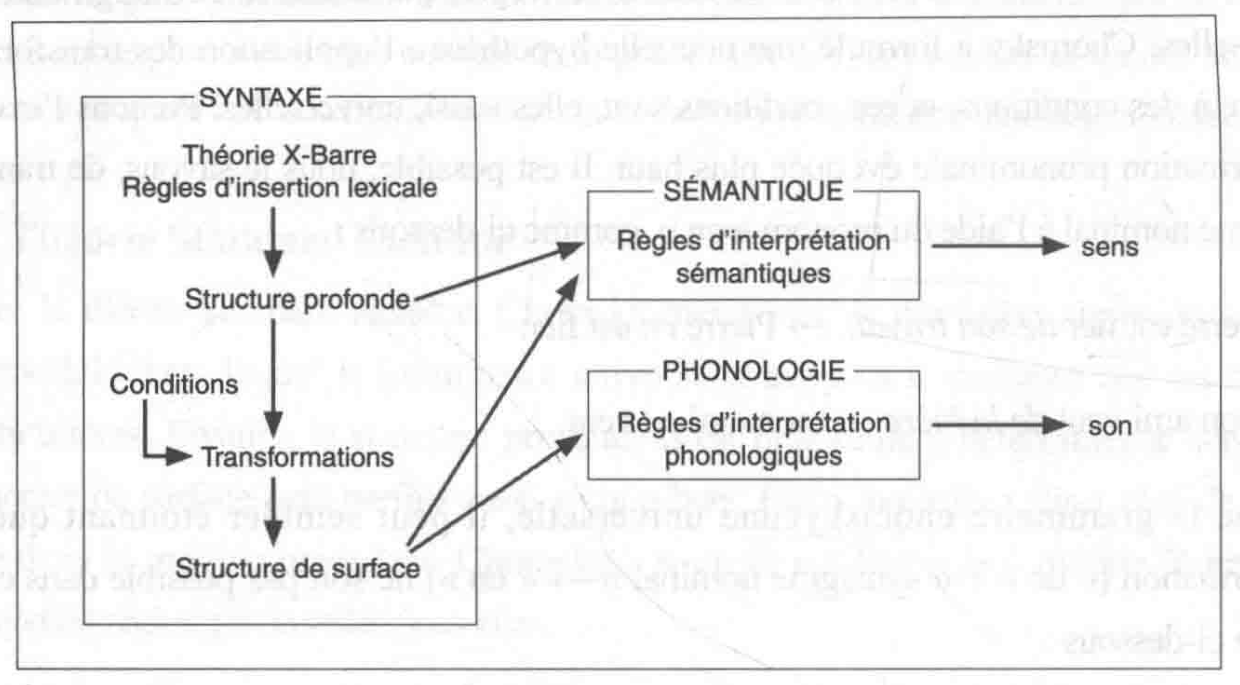
\includegraphics[width=.84\textwidth,height=.34\textheight,keepaspectratio]{assets/v17_extended.png}\end{center}

Dans la théorie standard étendue, le processus génératif est constitué de règles dont l’application est limitée, nous venons de le voir, par des conditions universelles. Le problème, c’est que de telles conditions impliquent le fait que le processus génératif connaît des exceptions, ou du moins des cas particuliers. Or, cela, encore une fois, correspond peu à l’idée de la faculté universelle du langage. Chomsky a donc élaboré une troisième version de son modèle visant à remplacer un modèle fait de règles et d’exceptions par un modèle qui ne comporte aucune exception. Ce nouveau modèle, basé d’une part sur des principes universels et d’autre part sur des paramètres spécifiques à chaque langue, est appelé « Principes et Paramètres » ( Principles and Parameters ).\par

\subsection{Les Principes et Paramètres (P\&P)}

Cette troisième version du processus génératif, proposée par Chomsky au début des années 1980, ne se limite pas, comme dans la théorie standard étendue, à apporter quelques modifications à la version précédente : elle constitue une véritable rupture. En se fixant comme objectif de dégager les propriétés universelles (Principes) des langues naturelles et leurs spécificités individuelles (Paramètres), la grammaire générative devient une théorie de la faculté de langage.\par

\origpage{457}{443}

\minititle{\textcircled{\scriptsize 1} Lectures on Government and Binding}
Parmi les « principes » universels évoqués plus haut, on cite fréquemment la « théorie du gouvernement et du liage », exposée en 1981 dans Lectures on Government and Binding, traduit en 1991 sous le titre de « Théorie du gouvernement et du liage ». Cet essai de 1981 a été suivi un an plus tard de Some Concepts and Consequences of the Theory of Government and Binding, traduit en 1987 sous le titre de « La Nouvelle Syntaxe ».\par

\minititle{1. Liage et catégorie gouvernante}

La théorie du liage concerne la coréférence des pronoms et des anaphores (pronoms réfléchis et réciproques dans la grammaire traditionnelle). Par « coréférence », on entend le phénomène qui consiste pour plusieurs expressions différentes contenues dans une phrase à désigner le même objet, comme dans l’exemple ci-dessous :\par

\noindent\textbf{Ex :} Pierre sait que Paul /e reconnaît.\par

Ici, le pronom « le » ne peut coréférer qu’avec « Pierre », et pas avec « Paul ».\ednote{La contrainte locale interdit surtout que \textit{le} soit lié par le sujet local \textit{Paul}. Le pronom peut en principe renvoyer à Pierre ou à un référent discursif extérieur ; « qu’avec Pierre » est donc trop restrictif.} Ex : Pierre sait que Paul se reconnaît.\par

Dans l’exemple ci-dessus, par contre, l’anaphore réflexive (« se ») ne peut coréférer qu’avec « Paul », et pas avec « Pierre ». Pour comprendre la raison de cette différence, il faut partir des structures simplifiées :\par

Pierre sait (que Paul /e reconnaît.) © Pierre sait (que Paul se reconnaît.)\par

Dans les deux cas, le pronom « le » et l’anaphore « se » sont insérés dans un ensemble constitué par les deux parenthèses et qu’on appelle leur « catégorie gouvernante » (d’où le nom de théorie du gouvernement et liage). Or, selon le principe qui régit le phénomène de coréférence :\par

Un pronom ne peut être lié qu’à l'extérieur de sa catégorie gouvernante. © Une anaphore ne peut être liée qu’à l’intérieur de sa catégorie gouvernante. 2. Les trois principes du liage\par

La théorie du liage se fonde sur trois principes selon les trois différents syntagmes nominaux concernés : anaphore, pronom et expression référentielle (c’est-à-dire les noms communs et noms propres).\par

\minititle{1) Le principe A : l’anaphore}

Selon ce principe, une anaphore doit être liée dans sa catégorie gouvernante. Autrement dit, une anaphore doit avoir un antécédent local proche :\par

\noindent\textbf{Ex :} John washed himself.\par

\origpage{458}{444}

L’exemple ci-dessus respecte le principe A : l’antécédent de himself, c’est-à-dire John, est proche, et tous deux coréfèrent à la personne.\par

\noindent\textbf{Ex :} *(John asked Mary) to wash himself:\par

Cette phrase n’est pas acceptable car le réflexif himself se trouve hors dans sa catégorie gouvernante : réflexif et antécédent sont donc trop éloignés l’un de l’autre.\par

\minititle{2) Le principe B : le pronom}

Selon ce second principe, les pronoms sont libres de toute coréférence dans leur catégorie gouvernante. Cela veut dire qu’un pronom peut avoir un antécédent à condition que cet antécédent ne soit pas local et soit en quelque sorte éloigné. Ex : (John asked Mary) to wash him.\par

John est l’antécédent de him, et him est suffisamment éloigné de John : le principe B est respecte.\par

\noindent\textbf{Ex :} *John washed him.\par

L’exemple ci-dessus n’est pas acceptable car pronom et antécédent sont trop proches. En revanche, dans l’exemple ci-dessous, le principe B est respecté :\par

\noindent\textbf{Ex :} (Bébé est malade), la maman /e soigne.\par

Le pronom « le » qui obéit au principe B du liage, puisque son antécédent se trouve en dehors de sa catégorie gouvernante, séparé à l’écrit par une virgule et par une pause à l’oral.\par

\minititle{3) Le principe C : l’expression référentielle}

Ce principe indique qu’une expression référentielle (R-expression), c’est-à-dire un mot ou groupe de mots sémantiquement autonomes, ne peut pas avoir d’antécédent qui le commande.\ednote{Dans la théorie du liage, le principe C est usuellement formulé ainsi : une expression R doit être libre, c’est-à-dire ne pas être liée par un antécédent co-indexé qui la c-commande. Le verbe « commande » du texte est donc trop vague et peut inverser la relation pertinente.} Prenons quelques exemples :\par

\noindent\textbf{Ex. 1 :} Pierre ; aime son, , chien.\par

Dans ce premier exemple, l’adjectif possessif « son » peut librement référer à Pierre (référent 1) ou à quelqu’un d’autre (référent 2). Pierre est assez haut dans la structure pour qu’il n’y ait aucun risque que le possessif « son » soit plus haut que lui dans la structure.\par

\noindent\textbf{Ex. 2 :} * Son, , chien aime Pierre ,.\par

Dans l’exemple 2, le possessif est plus haut dans la structure que l’expression référentielle Pierre. Il n’est donc plus possible de lire la phrase avec la même liberté qu’en l’exemple 1 : le possesseur du chien est forcément quelqu’un d’autre que Pierre. Le principe C interdit la coréférence du possessif et de Pierre : on dira que le possessif « c-commande » l’expression référentielle Pierre.\par

\origpage{459}{445}

\noindent\textbf{Ex. 3 :} *Il, , aime le chien de Pierre ,.\par

C’est la même chose dans l’exemple 3, où en vertu de même principe le pronom i/ ne peut pas co-référer avec Pierre. Autrement dit, i/ ne peut pas être Pierre.\par

\minititle{\textcircled{\scriptsize 2} La théorie des Barrières (subjacency theory)}
Un autre exemple de Principe et Paramètres souvent cité est la théorie des barrières (ou des bornes), appelée subjacency theory en anglais. Selon ce principe, lorsqu’on déplace un constituant dans une phrase, le constituant déplacé laisse sur son « site d’extraction » (c’est-à-dire sa position dans la phrase avant qu’il ne soit déplacé) une catégorie vide identique. Cette catégorie vide, non- lexicale et non sémantique, est appelée « trace », un peu comme des traces de pas dans la neige. Le constituant déplacé est appelé « antécédent de la trace ».\par

La théorie des barrières stipule les conditions limitant la distance entre un antécédent (constituant déplacé) et une catégorie vide (sa trace) : selon le principe de sous-jacence, la distance entre un antécédent et sa trace ne peut dépasser une certaine distance, mesurée en « bornes ». Cette théorie concerne en particulier les « mots en QU » en français (« qui », « que », « quand », etc.) et les\par

« mots en WH » en anglais, comme « who » « which », « where », « when », etc. 1. Le mouvement Qu (WH-movement)\par

Le « déplacement QU » est une transformation syntaxique qui concerne le mouvement des syntagmes interrogatifs. Cette opération est appelée « déplacement QU » parce que plusieurs mots interrogatifs français, on vient de le voir, commencent par « qu- » Il existe en français d’autres mots interrogatifs qui ne commencent pas « qu » mais qui sont néanmoins soumis au déplacement QU : pourquoi, comment, combien, où.\par

En anglais, cette opération est appelée « wh-movement » pour la même raison : les mots interrogatifs anglais commencent typiquement par « wh- ». Prenons à présent quelques exemples pour illustrer cette théorie :\par

\noindent\textbf{Ex :} Tom has been reading Tesnière. Who has Tom been reading?\par

\noindent\textbf{Ex :} He should stop talking about syntax. What should he stop talking about?\par

\noindent\textbf{Ex :} They want to visit us tomorrow. When do they want to visit us?\par

En anglais comme en français aussi, le déplacement se fait selon un ordre particulier, et le syntagme interrogatif se trouve en début de phrase : c’est ce qu’on appelle en anglais « Wh- fronting » ou « Wh extraction ». Regardons à présent un autre exemple :\par

\origpage{460}{446}

\noindent\textbf{Ex :} Tu crois que Paul déteste qui ?\par

La structure profonde ci-dessus subit une transformation de type Wh-fronting et donne la structure de surface suivante :\par

\noindent\textbf{Ex :} Qui crois-tu que Paul déteste ?\par

Pourtant, dans certains cas, ce mécanisme est bloqué. Regardons la structure profonde simplifiée suivante : Ex : Crois-tu [la rumeur (que Paul déteste qui) ?]\par

Dans ce cas précis, la transformation interrogative est bloquée et le syntagme interrogatif « qui » ne pourra pas se déplacer en début de phrase : |\par

\noindent\textbf{Ex :} *Qui crois-tu [la rumeur (que Paul déteste) ?] Pourquoi cela ? Pour y répondre, Chomsky fait appel au principe de la sous-jacence. 2. Sous-jacence et îlots syntaxiques (Wh islands)\par

En syntaxe générative, les déplacements de composants sont soumis, on l’a vu, à des contraintes. Dans l’exemple ci-dessous, la proposition entre parenthèses est appelée « domaine sous-jacent », c’est-à-dire sous-jacent à la proposition qui lui est supérieure :\par

\noindent\textbf{Ex :} tu penses (que Paul épousera qui) ?\par

Après transformation interrogative et Wh-fronting, cette structure profonde va donner la structure de surface suivante :\par

\noindent\textbf{Ex :} Qui penses-tu que Paul épousera ?\par

Dans ce cas, on peut extraire « qui » de son domaine. Si le déplacement est possible, c’est parce que « qui » ne franchit qu’une seule borne (appelée aussi « barrière ») de domaine, autrement dit une seule parenthèse. La distance entre l’antécédent et sa trace est d’une borne seulement. Revenons à présent sur l’exemple vu un peu plus haut :\par

\noindent\textbf{Ex :} Crois-tu [la rumeur (que Paul épousera qui)] ?\par

Dans ce cas, on ne peut pas extraire « qui » de son domaine, car le mot interrogatif « qui » devrait franchir deux bornes, et la distance entre l’antécédent et sa trace serait trop importante :\par

\noindent\textbf{Ex :} *Qui crois-tu [la rumeur (que Paul épousera)] ? C’est la même chose avec l’exemple ci-dessous : Ex : John wonders [where Eric went (to buy a gift).]\par

« What does John wonder where Eric went to buy » est incorrect, et l'extraction est bloquée pour\par

\origpage{461}{447}

les raisons évoquées plus haut.\par

Le linguiste américain John Ross (1938-), ancien élève de Harris et de Chomsky s’est intéressé à ce genre de phrases qu’il appelle des îlots syntaxiques (extraction islands ou syntactic islands).\par

\minititle{\textcircled{\scriptsize 3} P-structure et S-structure}

La mise à jour de nouveaux principes tels que la coréférence ou la sous-jacence a été accompagnée d’une simplification de la notion de transformation. Dans les versions précédentes, le processus génératif comportait de nombreuses transformations parfois communes à toutes langues mais le plus souvent spécifiques à chacune, donc non universelles. Les études conduites par Chomsky dans le cadre des Principes et Paramètres ont permis de montrer que les transformations impliquent toutes des déplacements, comme nous venons de le voir. Chomsky a donc réduit le processus génératif à deux étapes :\par

Dans premier temps, il applique la théorie X-barres universelle à des mots du lexique pour former une P-Structure (la structure profonde de l’ancien modèle),\par

Dans un deuxième temps, il applique à cette P-Structure des mouvements pour engendrer une S-Structure (la structure de surface de l’ancien modèle)\par

La P-structure regroupe les éléments qui permettent de donner à la phrase une « forme logique ». La S-structure, quant à elle, regroupe les éléments nécessaires à la prononciation de la phrase, et qui lui donnent une « forme phonétique ».\par

\minititle{\textcircled{\scriptsize 4} Modules intentionnel-conceptuel et sensori-moteur}

A ce stade de la présentation de la troisième version et avant d’aller plus loin, je dois préciser que la faculté de langage selon Chomsky est régie par le cerveau. Selon cette conception, le cerveau comporte deux modules spécialisés qui interagissent l’un avec l’autre : le module sensori-moteur et le module intentionnel-conceptuel. Le module central transfère l’information contenue dans la forme logique au module intentionnel-conceptuel du cerveau, et transfère les informations de la forme phonétique au module sensori-moteur. Dans Three Factors in Language Design (2005), Chomsky précise cette terminologie :\par


\begin{lecture}{Extrait}
Dans notre terminologie, les expressions générées par un langage doivent satisfaire deux conditions d'interface : celles qu’impose le système sensori-moteur (SM) et celles qu'impose le système conceptuel intentionnel (C-I) qui entre dans la capacité intellectuelle humaine et dans la variété des actes de langage.
\end{lecture}
 Je vous invite à présent à comparer le cadre des principes et paramètres résumé dans le schéma ci-dessous, avec celui des deux versions précédentes. J’attire votre attention sur l’ajout de la théorie X-barres, la disparition des transformations, l’apparition du mouvement et des principes et paramètres qui le régissent, et, très important, l’apparition des deux modules (interfaces) spécialisés de la fonction langagière.\par

\origpage{462}{448}

\begin{center}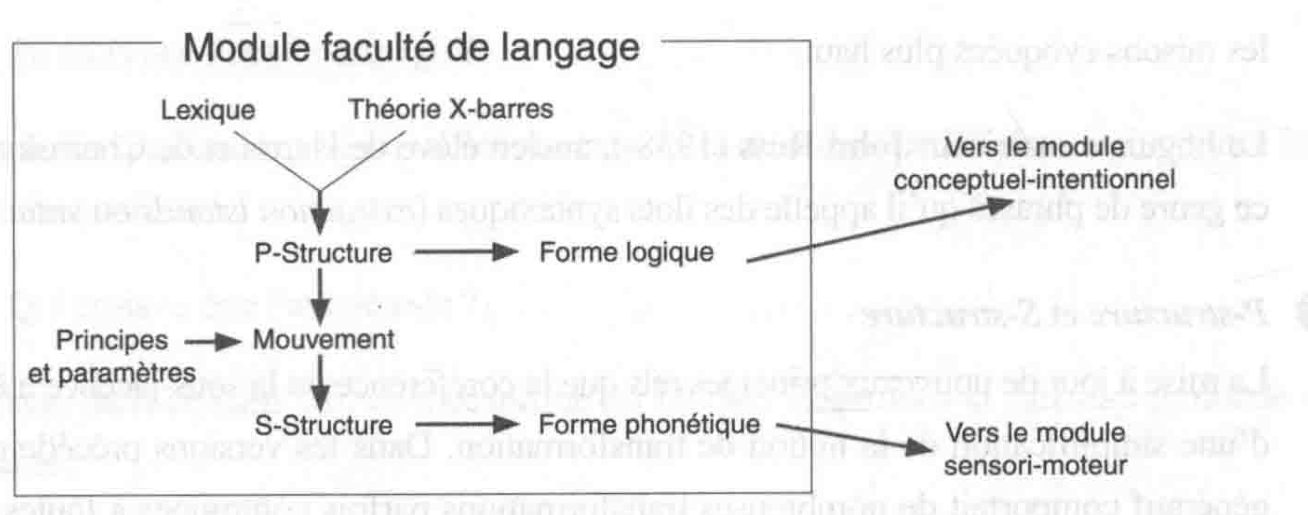
\includegraphics[width=.84\textwidth,height=.34\textheight,keepaspectratio]{assets/v17_pp.png}\end{center}

\subsection{Le programme minimaliste (Minimalist Program)}

Le Minimalist Program (1993, puis 1995) de Chomsky, est l’aboutissement d’une longue « errance générative », pour reprendre ses propres mots, commencée en 1957 par la parution de Syntactic structures, suivie de Standard Theory (1964-1967), de la Extended Standard Theory (1967-1977), Revised Extended Standard Theory (1977-1979), Theory of Government and Binding et Principes and Parameters (1980).\par

Ce programme minimaliste, dernière révision du modèle génératif, n’est pas fondé sur le constat d’un échec ou d’une insuffisance des Principes et Paramètres, mais sur l’adoption d’une toute nouvelle hypothèse : celle de l’optimalité de la faculté de langage. Partant de ce principe, Chomsky fonde son nouveau modèle sur un « principe d'économie » : pour être optimale, la grammaire ne doit rien comporter qui ne soit utile à sa fonction, à savoir engendrer des suites de mots dotées de sons et de sens.\par

Avec ce programme minimaliste, la grammaire générative devient de plus en plus abstraite, Les niveaux de représentations se limitent à la forme phonologique (PF) et la forme logique (LF). La D-Structure est remplacée par l’opération de fusion (merging), la S-Structure est remplacée par l’opération d’épellation (spell-out).\ednote{Dans le programme minimaliste, D-Structure et S-Structure sont éliminées comme niveaux de représentation. \textit{Merge} construit les objets syntaxiques et \textit{Spell-Out} transfère une dérivation vers les interfaces ; parler de remplacement terme à terme simplifie excessivement le changement de modèle.} Quant à la notion de competence, elle est remplacée par le langage interne (/-language).\par

\minititle{\textcircled{\scriptsize 1} La numération}
La dérivation d’une phrase commence par la sélection des items lexicaux (autrement dit, du lexique) syntaxiquement compatibles et nécessaires à sa construction. L’ensemble des items ainsi sélectionnés est appelé numération. Une fois ces éléments sélectionnés, deux opérations majeures interviennent dans la construction des énoncés : la Fusion et le Déplacement.\par

\minititle{\textcircled{\scriptsize 2} La fusion (merge)}
L'opération de fusion consiste à combiner deux éléments de l’énumération ci-dessus pour en engendrer un troisième, puis faire de même avec deux autres mots, puis encore deux autres, etc. jusqu’à l’épuisement de l’énumération : cette opération est récursive (itérative), c’est-à-dire qu’elle est répétée autant de fois qu’il y a d’éléments dans l’énumération. Dans le modèle minimaliste, ce sont ces opérations de fusion successives qui engendrent la structure de base. Chomsky distingue deux cas de fusion :\par



\origpage{463}{449}

on peut fusionner B avec A depuis l'extérieur de A : c’est la fusion externe (external merge),\par

on peut fusionner aussi B avec A depuis l’intérieur de A : c’est la fusion interne (internal merge), appelée aussi déplacement (move).\par

\minititle{\textcircled{\scriptsize 3} Le déplacement (move) et la vérification (feature-checking)}

Motivé par la nécessité de vérifier certains traits (feature-checking), le Déplacement (move) est la troisième opération de dérivation du programme minimaliste. La condition de pleine interprétation (full interpretation) qui régit les niveaux PF et LF exige en effet que tout trait soit interprétable, c’est-à-dire bien formé. Si c’est le cas, il sera alors transféré, comme on l’a vu plus haut, dans l’interface phonologique pour une réalisation phonétique. Si au contraire il est mal formé, il sera éliminé.\par

\minititle{④ L’épellation (spell-out)}

Lorsque tous les éléments de l’énoncé ont atteint leur position de surface, c’est-à-dire au moment où ils doivent être prononcés, le Spell-Out, point de transfert vers les deux interfaces, va intervenir et séparer la forme phonologique (PF) de la forme logique (LF), comme résumé dans le schéma ci-dessous :\par

\begin{center}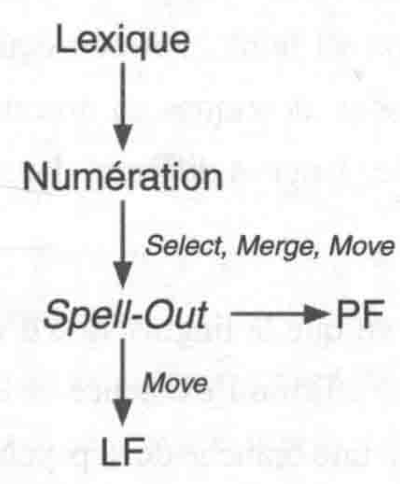
\includegraphics[width=.84\textwidth,height=.34\textheight,keepaspectratio]{assets/v17_spellout.png}\end{center}

C’est cette opération de Spell-out qui explique pourquoi, alors que la structure de base des énoncés est universelle, leur forme phonologique diffère d’une langue à l’autre : elle dépend du moment où le Spell-out a lieu. Selon le modèle minimaliste, les variations entre les langues sont en effet la conséquence d’une variation du moment où l’épellation a lieu. Ainsi, dans certaines langues, certains déplacements (fusion interne) ont lieu avant le Spell-out, tandis que dans d’autres langues, ils ont lieu après : c’est cela qui, pour Chomsky, qui explique la différence dans l’ordre des mots.\par

Si on l’interroge à présent sur le « pourquoi » de cette différence dans le moment du déplacement, Chomsky répond que cela est dû à l’existence de deux types de traits formels : des traits forts et des traits faibles :\par

Les traits forts doivent être vérifiés avant l’Épellation : le résultat est visible dans la forme phonologique.\par

Les traits faibles peuvent être vérifiés après l’Épellation : le résultat est invisible dans la forme phonologique.\par



\origpage{464}{450}

Quant à la force d’un trait, elle dépend de la langue en question. Pour illustrer cela, prenons quelques exemples en anglais et en français, et comparons la position du verbe par rapport à la négation, et par rapport à l’adverbe, et cela au présent comme au passé composé : Ex. 1 : Jean ne dort pas. John does not sleep. Ex. 2 : Jean n’a pas dormi. John did not sleep. Ex. 3 : Jean embrasse souvent Marie. John often kisses Mary. Ex. 4 : Jean a souvent embrassé Marie. John ofien kissed Mary.\ednote{« ofien » est une coquille pour \textit{often}. De plus, le prétérit \textit{kissed} ne correspond pas au présent de « Jean embrasse souvent Marie » ; la phrase parallèle attendue serait « John often kisses Mary ».}\par

On remarque qu’en français, le mouvement du verbe a lieu avant le Spell-out en français mais après : cela est dû au fait que les verbes français sont dotés d’un trait formel fort et que les verbes anglais sont dotés d’un trait formel faible. Par conséquent, les deux langues diffèrent sur le plan phonologique, alors qu’elles sont identiques au niveau de la forme logique. Retenez donc que, selon le modèle minimaliste, les langues diffèrent dans la force des traits formels qui composent leurs items lexicaux.\par

Dans ce chapitre, nous avons vu que la linguistique d’inspiration chomskyenne, qui se proclame mentaliste et anti-béhavioriste, affirme l’existence et la prééminence des activités mentales. La linguistique, pour Chomsky, est une branche de la psychologie. Par ailleurs, en intégrant le cerveau et l’esprit dans la réflexion linguistique, en postulant l’existence d’un organe langagier, et en soutenant que la capacité langagière présente chez l’homme a un fondement biologique, Chomsky a pris une orientation qu’il qualifie lui-même de biolinguistique.\par

\origpage{465}{451}
\section*{Exercices}
\addcontentsline{toc}{section}{Exercices — chapitre 14}
\begin{keybox}[I]
\textbf{Dans cet extrait de \textit{Aspects of the Theory of Syntax} (1965), quelles critiques Chomsky adresse-t-il aux grammaires traditionnelles et à la linguistique moderne ? Quel est l’argument de Du Marsais ? Quel rapprochement pouvez-vous faire avec la grammaire Port-Royal ? Comment Diderot explique-t-il l’ordre des mots en français ? Qu’en conclut Chomsky ?}

\begin{lecture}{Aspects of the Theory of Syntax (1965)}
Languages, therefore, resemble men in this respect, that, though each has peculiarities, whereby it is distinguished from every other, yet all have certain qualities in common. The peculiarities of individual tongues are explained in their respective grammars and dictionaries. Those things, that all languages have in common, or that are necessary to every language, are treated of in a science, which some have called Universal or Philosophical grammar. Somewhat earlier, Du Marsais defines universal and particular grammar in the following way (1729; quoted in Sahlin, 1928, pp. 29-30):

Il y a dans la grammaire des observations qui conviennent à toutes les langues ; ces observations forment ce qu’on appelle la grammaire globale : telles sont les remarques que l’on a faites sur les sons articulés, sur les lettres qui sont les signes de ces sons ; sur la nature des mots, et sur les différentes manières dont ils doivent être ou arrangés ou terminés pour faire un sens. Outre ces observations générales, il y en a qui ne sont propres qu’à une langue particulière ; et c’est ce qui forme les grammaires particulières de chaque langue.

Modern linguistics, however, has not explicitly recognized the necessity for supplementing a “particular grammar” of a language by a universal grammar if it is to achieve descriptive adequacy. It has, in fact, characteristically rejected the study of universal grammar as misguided; and, as noted before, it has not attempted to deal with the creative aspect of language use.

Another reason for the failure of traditional grammars, particular or universal, to attempt a precise statement of regular processes of sentence formation and sentence interpretation lay in the widely held belief that there is a “natural order of thoughts” that is mirrored by the order of words. Hence, the rules of sentence formation do not really belong to grammar but to some other subject in which the “order of thoughts” is studied. Thus in the \textit{Grammaire générale et raisonnée} (Lancelot sequence of words follows an “ordre naturel,” which conforms “à l’expression naturelle de nos pensées.” Consequently, few grammatical rules need be formulated beyond the rules of ellipsis, inversion, and so on, which determine the figurative use of language. The same view appears in many forms and variants. To mention just one additional example, in an interesting essay devoted largely to the question of how the simultaneous and sequential array of ideas is reflected in the order of words, Diderot concludes that French is unique among languages in the degree to which the order of words corresponds to the natural order of thoughts and ideas (Diderot, 1751). Thus « quel que soit l’ordre des termes dans une langue ancienne ou moderne, l’esprit de l’écrivain a suivi l’ordre didactique de la syntaxe française » (p. 390):
\end{lecture}
\origpage{466}{452}
\begin{lecture}{Suite}
« Nous disons les choses en français, comme l’esprit est forcé de les considérer en quelque langue qu’on écrive » (p. 371). With admirable consistency he goes on to conclude that « notre langue pédestre a sur les autres l’avantage de l’utile sur l’agréable » (p. 372); thus French is appropriate for the sciences, whereas Greek, Latin, Italian, and English « sont plus avantageuses pour les lettres. » Moreover :

Le bons sens choisirait la langue française ; mais l’imagination et les passions donneront la préférence aux langues anciennes et à celles de nos voisins il faut parler français dans la société et dans les écoles de philosophie ; et grec, latin, anglais, dans les chaires et sur les théâtres ; notre langue sera celle de la vérité, si jamais elle revient sur la terre ; et la grecque, la latine et les autres seront les langues de la fable et du mensonge.

Le français est fait pour instruire, éclairer et convaincre; le grec, le latin, l’italien, l’anglais, pour persuader, émouvoir et tromper : parlez grec, latin, italien au peuple ; mais parlez français au sage. (pp. 371-3721)\ednote{La référence finale « pp. 371-3721 » comporte manifestement un chiffre surnuméraire ; l’intervalle attendu est pp. 371-372. Le corps du texte est laissé tel quel.}

In any event, insofar as the order of words is determined by factors independent of language, it is not necessary to describe it in a particular or universal grammar, and we therefore have principled grounds for excluding an explicit formulation of syntactic processes from grammar.
\end{lecture}
\end{keybox}

\begin{keybox}[II]
\textbf{Réalisez les arbres syntaxiques des phrases suivantes :}
\begin{enumerate}
\item Parler de la violence à la télévision.
\item L’enfant joue à la balle dans le jardin.
\item L’oiseau pose ses pattes sur une branche.
\item Colourless green ideas sleep furiously.
\item Times flies like an arrow.\ednote{La maxime grammaticale célèbre est « Time flies like an arrow ». Le pluriel \textit{Times} du texte de base paraît être une coquille.}
\item Remember in prayer the one who are sick in our church.\ednote{原文如此。one 与 are 数不一致；应按所指改为 the one who is 或 the ones who are。保留原题，不代作练习。}
\item Buffalo buffalo Buffalo buffalo buffalo buffalo Buffalo buffalo.
\item John told the little boy he won the prize.
\item The little boy has broken the toy.
\item The angry bear chased the frightened little squirrel.
\end{enumerate}
\end{keybox}

\begin{keybox}[III]
\textbf{Traduisez en mandarin les phrases ambiguës suivantes (deux sens possibles) :}
\begin{enumerate}
\item Le policier a abattu un homme avec son arme.
\item La petite brise la porte.
\item Je me suis rendu au commissariat de police.
\item Je l’ai vue avec une nouvelle paire de lunettes.
\item Ils m’ont rapporté des fruits d’Afrique.
\item Je crois cet enfant honnête.
\item J’aime bien ce portrait de Picasso.
\item Cette critique de Proust est bien sévère !
\item Flying planes can be dangerous.
\item I shot an elephant in my pyjamas.
\end{enumerate}
\end{keybox}

\origpage{467}{453}
\begin{keybox}[IV]
\textbf{Traduisez en mandarin chacune des deux structures représentées dans les arbres syntaxiques suivants :}
\begin{center}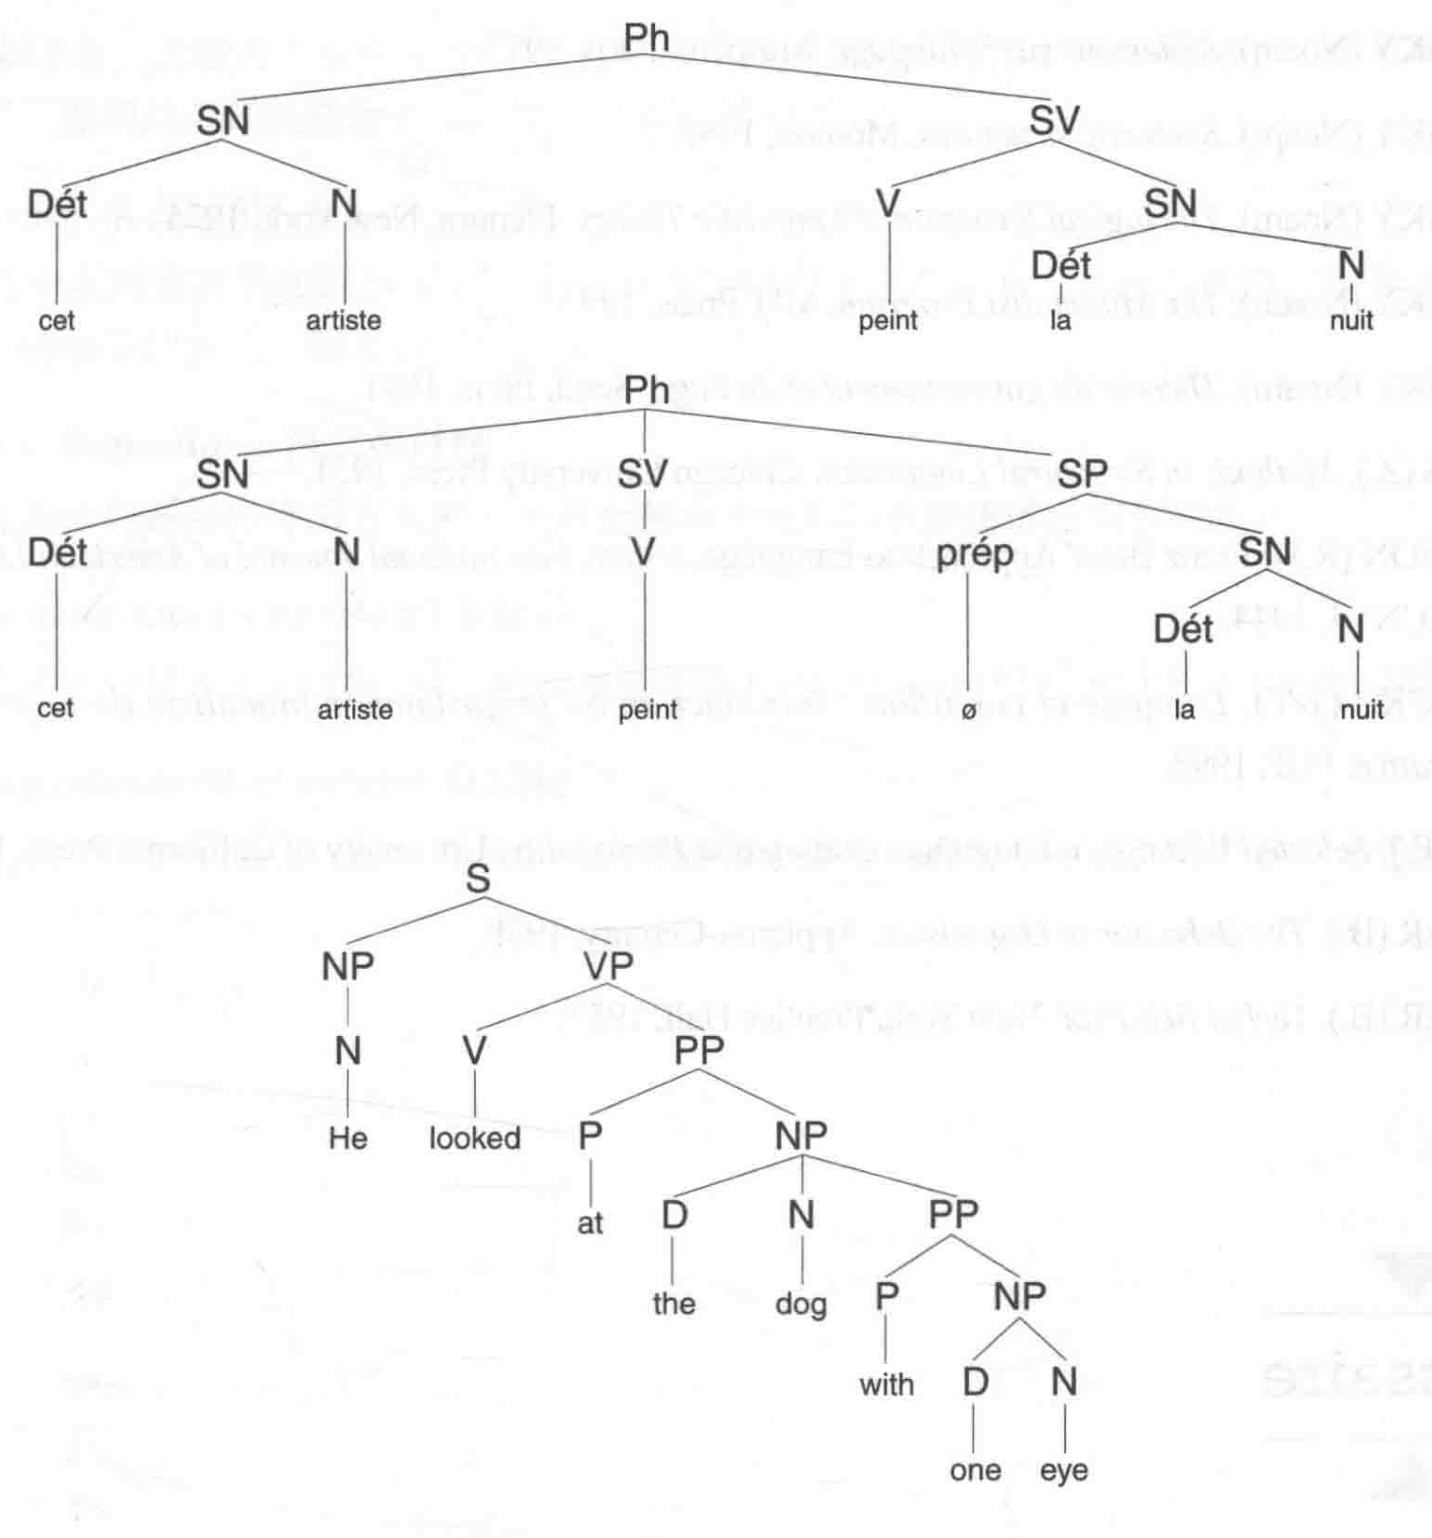
\includegraphics[width=.84\textwidth,height=.50\textheight,keepaspectratio]{assets/v17_exercises.png}\end{center}
\end{keybox}

\section*{Pour aller plus loin}
\addcontentsline{toc}{section}{Pour aller plus loin — chapitre 14}
\begin{small}
\begin{description}[style=nextline,leftmargin=0pt,labelindent=0pt]
\item[BLOOMFIELD (L.).] \textit{Le Langage.} Paris, Payot, 1970.
\item[BOLTANSKI (J.-E.).] \textit{La révolution chomskyenne et le langage.} L’Harmattan, 2002.
\item[CHOMSKY (Noam).] \textit{Aspects de la théorie syntaxique.} Seuil, Paris, 1971.
\item[CHOMSKY (Noam).] \textit{Essays on Form and Interpretation.} North Holland, Elsevier, 1977, trad. française \textit{Essais sur la forme et le sens}, Seuil, Paris, 1980.
\origpage{468}{454}
\item[CHOMSKY (Noam).] \textit{Nouveaux horizons dans l’étude du langage et de l’esprit.} Stock, 2005.
\item[CHOMSKY (Noam).] \textit{Réflexions sur le langage.} Maspéro, Paris, 1977.
\item[CHOMSKY (Noam).] \textit{Syntactic Structures.} Mouton, 1957.
\item[CHOMSKY (Noam).] \textit{The Logical Structure of Linguistic Theory.} Plenum, New York, 1975.
\item[CHOMSKY (Noam).] \textit{The Minimalist Program.} MIT Press, 1995.
\item[CHOMSKY (Noam).] \textit{Théorie du gouvernement et du liage.} Seuil, Paris, 1991.
\item[HARRIS (Z.).] \textit{Methods in Structural Linguistics.} Chicago University Press, 1951.
\item[JAKOBSON (R.).] « Franz Boas’ Approach to Language. » dans \textit{International Journal of American Linguistics}, vol. 10, no 4, 1944.
\item[POLLOCKP (J.-Y.).] \textit{Langage et cognition : introduction au programme minimaliste de la grammaire générative.} PUF, 1998.\ednote{Le nom de l’auteur est imprimé « POLLOCKP » dans le fond. Il s’agit de Jean-Yves Pollock ; le second P est une coquille.}
\item[SAPIR (E.).] \textit{Selected Writings in Language, Culture and Personality.} University of California Press, 1985.
\item[SKINNER (B.).] \textit{The Behavior of Organisms.} Appleton-Century, 1938.
\item[SKINNER (B.).] \textit{Verbal Behavior.} New York, Prentice Hall, 1957.
\end{description}
\end{small}

\section*{Glossaire}
\addcontentsline{toc}{section}{Glossaire — chapitre 14}
\gloss{behaviorisme}{行为主义}{心理学的一个理论，说明人和动物的行为只能且必须从物质过程的角度来研究，不用参考心智。受它影响产生的学习理论解释了在不断强化下个体是如何受外部事件影响而产生行为变化的。一些学者用行为主义解释第一语言的习得。}
\gloss{compétence}{语言能力}{生成语法中组成一个人语言知识的内化规则系统，它包括人能够理解并说出句子，包括从来没听过的句子的能力；某一特点语言中什么是句子什么不是句子的知识和区分歧义及区别偏离语法规则的句子的能力。}
\gloss{distributionnalisme/analyse distributionnelle}{分布分析法}{特定语言单位出现的位置的范围称分布。该方法分析语言诸单位在语言结构中的分布关系，借以进行语言单位的分类与归纳语言的结构系统。}
\origpage{469}{455}
\gloss{grammaire générative}{生成语法}{一种语法理论，试图用一套规则定义和描写某一种语言中所有合乎语法的句子，而不包括不合法的句子。据说这类语法能生成或产生合乎语法的句子。}
\gloss{performance}{语言运用}{生成语法中人对语言的实际运用。一个人的语言知识（语言能力）不同于他用这种知识来造成句子和理解句子的方式（语言运用）。}
\gloss{relativisme linguistique}{语言相对性}{该观点认为人们看待世界的方法部分地或全部地为他们的本族语的结构所决定。}
\gloss{structure de surface (S-structure)}{S 结构}{句子形式的下一层次为 S 结构，这一层次被授予各种句法／语法的格，如主格／主语和受格／宾语。}
\gloss{structure profonde (D-structure)}{D 结构}{句子形式的一种抽象层次，句子在这一层次里被授予如施动者和受事者这样的语义角色。}
